
%% Note: If you are using this template for a proposal, pass the proposal option to
%% the class.  Then the toplevel section will be \section, not \chapter.  In either case
%% the \appendix command, which should only be used in the EndMatter environment, can be considered
%% to be at the same toplevel (either section or chapter}.

%% NOTE: Hyperref package doesn't yet completely work with the proposal option.  It compiles
%% but the pdf bookmarks aren't correct.

%% Please report bugs/problems to djallred@gmail.com

%% Begin Preamble Info
\documentclass[12pt,letterpaper,doublespaced,ETD,dvips,proposal]{gtthesis}

\title{Scalable Manifold Learning with Applications in Speech}
\author{Nikolaos Vasiloglou II}
\copyrightyear{2007}
\graddate{August 2007} %Appears at bottom of title page
\approvaldate{July 2007} %Appears on signature page (not needed for a proposal)

% Add people to signature list (not needed for a proposal)
\addadvisor{David Anderson}{Assoc. Professor, School of ECE}{Georgia
Institute of Technology}

\addadvisor{Alexander Gray}{Assist. Professor, School of CS}{Georgia
Institute of Technology}

\addchair{Dr. Sitting Bull}{Professor, School of ECE}{Georgia
Institute of Technology}

\addreader{Dr. Wayne Geronimo}{Asst. Professor, School of
ECE}{Georgia Institute of Technology}

\addreader{Dr. David Goliath}{Asst. Professor, School of
ECE}{Georgia Institute of Technology} \addreader{Dr. Marky
Mark}{Asst. Professor, School of ECE}{Georgia Institute of
Technology}

\addreader{Dr. Larry A. Stooge}{Asst. Professor, School of
ECE}{Georgia Institute of Technology}
\bibfiles{template}

%%Packages to use
\usepackage{graphicx}
\usepackage{insfig}
\usepackage{hyperref}
\usepackage{verbatim}
\usepackage{boxedminipage}

%%%% These commands set the default depth the TOC should be expanded
%%   out to for the chapters and appendices
%%
\setchaptertocdepth{2}
\setappendixtocdepth{2}

%%%% To rename different sections of the document use these
%%   set???string{ ...string...} commands where ??? is replaced
%%   by one of the following three letter codes
%%
%%   toc = table of contents   chp = chapter
%%   lof = list of figures     app = appendix
%%   lot = list of tables      prt = part (i.e. volume)
%%   bib = bibliography        abs = abstract
%%   ind = index               los = list of symbols
%%   ded = dedication          ack = acknowledgement
%%   glo = glossary,list of terms
%%
%%   Regardless of capitalization all will become capitalized in
%%   the final document.
%%
\settocstring{Table of Contents}
\setlofstring{List of Figures}
\setlotstring{List of Tables}
\setbibstring{References}
\setindstring{Index}
\setdedstring{Dedication}
\setglostring{List of Terms}
\setchpstring{Chapter}
\setappstring{Appendix}
\setprtstring{Volume}
\setabsstring{Summary}
\setlosstring{List of Symbols}
\setackstring{Acknowledgment}

%%%% Set the default page style for each main enviroment
%%
\setfrontpagestyle{plain}
\setbodypagestyle{plain}
\setendpagestyle{plain}

\begin{document}
\pagestyle{plain}

\begin{FrontMatter}
\contents %Generates the TOC, LOF, and LOT, glossary and LOS
%% Below are some optional environments that can be used here
\end{FrontMatter}

\begin{Body}
\section{Introduction}
\label{intro}The explosion of information over the last few decades has created data volumes of extraordinary size and dimensionality, 
bringing with it a great demand for analysis of and information extraction from these data.
Two approaches for analyzing these data are common in machine learning: parametric \cite{bishop2006pra, hastie2001esl, haykin1994nnc}
and non-parametric \cite{wasserman2006ans}. 
In parametric analysis there is an assumption of an underlying model and the model is estimated based on the data.  
In non-parametric analysis the data serves as the model.


%Information explosion during the last decades has
%created data volumes of extraordinary size and dimensionality. There
%is a great demand for analysis and information extraction from data.
%Two approaches are common in machine learning, the parametric one
%\cite{bishop2006pra, hastie2001esl, haykin1994nnc} and
%the non-parametric one \cite{wasserman2006ans}. In the parametric case there is an underlying model
%assumption. The concept is to estimate the model parameters given
%the data. In the non-parametric case the data is the model.

In the parametric case we start with a very large amount of data $N$
and we train a model that is described with $k$ parameters, where
$k<<N$. So evaluation of the model for new data is quite fast, since
it involves operations that have to do with $k$ parameters. In
practice, parametric models lead to non-convex optimization problems,
so it is difficult to find the best parameters given the data. The
most difficult part is to find the right number of the parameters
that best fit the data. For example the number of neurons and the
topology of a neural network is something that can only be
determined experimentally after testing different combinations given
a dataset. In any case the value of parametric models should not be
underestimated since it can achieve very good performance in
practice even if the best parameters have not been chosen.

In the parametric case the data is the model. The model has $N$
parameters plus one or two that have to be estimated. For example in
the Kernel Density Estimation problem \cite{Silverman}, the bandwidth $h$ of the
kernel has to be tuned, i.e.
\begin{equation}
\hat{f}(x)=\sum_{i}^{N}e^{-\frac{||x-x_i||}{h}}
\end{equation}
There are cases when the bandwidth depends on the point so the above
equation changes to
\begin{equation}
\hat{f}(x)=\sum_{i}^{N}e^{-\frac{||x-x_i||}{h_i}}
\end{equation}

\insfig[2d_kernel_density_estimation]{2d_kernel_density_estimation.eps}{Kernel
Density of 2 dimensional points. Over every point a kernel is set.
In areas with with high concentration of points there is more
overlap on the kernels which shows higher probability}{8cm}

In contrast to parametric cases, a single evaluation of a non
parametric model requires evaluation of $N$ parameters. Naively
speaking training can be avoided at all if the parameter is set
ad-hoc. If we want to find the single parameter with cross
validation then that would require $N^2$ operations per candidate
value of $h$. However if data are in a more sophisticated way
it is possible to reduce the training of the non-parametric model to
linear time and the evaluation of a new point in logarithmic time.
Estimation of the few parameters of a non-parametric model can be
casted as an optimization problem which in most of the cases can be
convex. In addition, the non-parametric Kernel Principal Component
Analysis \cite{scholkopf1998nca} can be computed with the help
of semidefinite programming \cite{vandenberghe1996sp, boyd2004co}.

\section{Origin and history of the problem}
\label{origin}

After the information explosion, the problem of reducing/estimating
the real dimensionality, also known as the intrinsic dimensionality of a
given dataset, has been an active area of research \cite{kegl2003ide}, \cite{costa2003egm}.
It is well known that many
machine learning algorithms starting from the very fundamental, the
nearest neighbor, grow exponentially on the intrinsic dimensionality of the data. This
is also known as the curse of dimensionality \cite{donoho2000hdd}.
In the literature, dimensionality is used without the prefix intrinsic or
extrinsic, causing confusion. The extrinsic dimensionality is just
the number of variables needed to describe a point, i.e. the
extrinsic dimensionality of $x\in \Re^d$ is just $d$. Each variable
of the d-dimensional vector will be called dimension $1\dots d$. In
reality, some of the dimensions might be linearly or non-linearly
dependent on other dimensions, thus fewer than $d$ dimensions are
sufficient to describe a point. We can define the intrinsic
dimensionality of a dataset as the minimum number of "independent"
variables needed to describe a point in space. Still the term is not
very clear, for the scope of this thesis we mean that there is no
algorithm that can predict a dimension from the others. Principal
Component Analysis for example \cite{jolliffe2002pca}, finds the most important dimensions
on a dataset that are linearly independent. In practice because of
noise all dimensions appear to be strictly independent.  Modern
kernel methods can capture non-lineal dependencies between
dimensions. Kernel PCA is the father of non-linear dimensionality
reduction methods \cite{scholkopf2002lks}.

Although Kernel PCA  seems to be a very powerful tool, it suffers from
polynomial complexity. It requires $O(N^2)$ kernel computations,
which make it unsuitable for large scale problems. In this thesis we
will show how  multidimensional trees can reduce
the complexity, along with other approximations to bring it down to
linear \cite{gray2000nbp}.

The driving force for investigating dimensionality reduction is the
estimation of the true dimensionality of speech. Many representations
have been recommended for speech including MFCC, LPC, NRAFF etc, \cite{quatieri2002dts,rabiner1978dps, ravindran:inr}, yet the true
dimensionality is unknown. Meanwhile there is theoretical evidence
that speech signals lie on manifolds
\cite{alder1991dss, sciamarella1999tsc, kumar1990ade, tishby1990dsa, jansen2006ifa}. In
this thesis we will attempt to estimate the true dimensionality of
speech based on several representations which may  help in developing new methods for speech
recognition.

\section{Preliminary Research}
\label{prelim}
\subsection{The Nearest Neighbor Problem}
\label{The_Nearest_Neighbor_Problem}

One of the classical problems in statistics and in machine learning
is the nearest neighbor problem. Given a set of points in $S =
\{x_i, x_i\in\Re^d, i=0\dots N\}$ and a distance metric $M(x_i, y_i),
x_i, y_i \in S$,  the nearest neighbor of $x_i \in \Re^d$ is
$argmin(M(x, y_i)), y_i \in S$. In many cases the problem of finding
all nearest neighbors appears. This problem can be formalized as
find $argmin(M(x, y_i)), y_i \in S, \forall x \in S'$. The problem
of finding nearest neighbor can be solved in a "naive" way, by
computing all the distances between the query point and the
reference points. The complexity is $O(N)$. Assuming that the number
of the query points $N$ is the same as the number of reference
points then the complexity of the naive method is $O(N^2)$. An
efficient way to reduce the complexity is to use multidimensional
trees. In the next sections we present kd-trees \cite{moore-tutorial}
and ball-trees \cite{moore2000ahu}.

As a clarification we mention that this is the problem of the exact
nearest neighbor. There are algorithms addressing the problem of
approximate neighbor. Local Sensitivity Hashing is one of the
algorithms that deal with this problem \cite{datar2004lsh}.

\subsubsection{Multidimensional Trees}
\label{Multidimensional_Trees}

The purpose of multidimensional trees is to create a hierarchical
partition of a dataset so that data points are grouped close to
their neighbors, which are usually the points of interest, and far
away enough from other points. It has been proven that there is not
a globally optimal partition strategy \cite{gyorfi2002dft}
and it is heavily dependant on the distribution of the data points
as well as on the dimensionality. In this section we present a particular
 class of multidimensional
trees, the binary trees and more specifically kd-trees and ball or
metric trees. The key concept in binary trees is partitioning a set
recursively in two sets at every step.

\subsubsection{Kd-trees}
\label{Kd_trees}

The first multidimensional tree in the literature was the kd-tree \cite{bentley1975bst}. After
30 years it still performs comparably and in some cases, even
better than modern trees. At every level a partition (pivot)
dimension is chosen according to a user defined criterion and the
data is split in two subsets according to this dimension. Kd-trees
are off-line trees. In order to build a kd-tree all the data must be
available before building the tree in contrast to other trees that
can dynamically add or delete points.

Several strategies have been recommended for finding the splitting
dimension. The most popular are splitting on the dimension with the
maximum variance or maximum range. However both of these strategies are heuristics and
there is no underlying theory behind them that guarantees better
performance of the trees. Another issue once the splitting dimension
is found, is the actual numeric value of the split value. In other words,
the ratio of the points going in the two resulting sets. The mid
value of the range or the mid value of the variance will in general
give two sets that in most of the cases will have different number
of points. Another strategy is to find the value that gives equally
sized sets. This strategy in general gives balanced trees, while the
first one leads to unbalanced trees. In the following sections we
show that empirically it is preferable to have unbalanced splits
on the tree, since it favors pruning in the process of finding the
nearest neighbors.

\paragraph{Data structures for kd-trees}

 Kd-trees consist of two types of data structures, nodes and
 leafs. The basic data needed for the nodes are the
 hyper-rectangles fig.~\ref{parent_kd_node}. Hyper-rectangles are the k-dimensional rectangles that describe the minimum bounding box  for a given set of points.
 Leafs hold the data points  fig.~\ref{2_kd_node}. The number of points on a
 leaf is user defined. The tree method for finding the nearest neighbor is faster than the naive
 only after a threshold of points. This threshold is used as the maximum number of points
 per leaf. Bounding boxes (Hyper-rectangles) and points are the minimum amount
 of information required to be stored on nodes on the leaf. Extra
 information about the data, such as the centroid of the box, higher
 order moments, etc also called Cached Statistics can speed up
 tremendously algorithms other than nearest neighbor. The algorithm
 of nearest neighbor search with kd-trees will be described  in the following section,
 fig.~\ref{nearest_neighbor_searchon_kd}.

\begin{figure}[!htb]
\label{parent_kd_node}
\centerline{\includegraphics[height=8cm]{parent_kd_node.eps}}
\caption{The parent node of a 2
dimensional kd-tree}
\end{figure}

%\insfig[parent_kd_node]{parent_kd_node.eps}{The parent node of a 2
%dimensional kd-tree}{8cm}

\begin{figure}[!htb]
\label{2_kd_node}
\centerline{\includegraphics[height=8cm]{2_kd_node.eps}}
\caption{A two node 2 dimensional
kd-tree}
\end{figure}

%\insfig[2_kd_node]{2_kd_node.eps}{A two node 2 dimensional
%kd-tree}{8cm}

\begin{figure}[!htb]
\label{nearest_neighbor_searchon_kd}
\centerline{\includegraphics[height=8cm]{nearest_neighbor_searchon_kd.eps}}
\caption{Nearest neighbor with pruning}
\end{figure}

%\insfig[nearest_neighbor_searchon_kd]{nearest_neighbor_searchon_kd.eps}{Nearest
%neighbor with pruning}{8cm}

\begin{figure}[!htb]
\label{nearest_neighbor_searchon_kd_true_neighbor}
\centerline{\includegraphics[height=8cm]{nearest_neighbor_searchon_kd_true_neighbor.eps}}
\caption{True nearest neighbor is out of the leaf}
\end{figure}

%\insfig[nearest_neighbor_searchon_kd_true_neighbor]{nearest_neighbor_searchon_kd_true_neighbor.eps}
%{True nearest neighbor is out of the leaf}{8cm}

\begin{figure}[!htb]
\label{nearest_neighbor_searchon_kd_no_prune}
\centerline{\includegraphics[height=8cm]{nearest_neighbor_searchon_kd_no_prune.eps}}
\caption{Kd tree with no possible pruning}
\end{figure}

%\insfig[nearest_neighbor_searchon_kd_no_prune]{nearest_neighbor_searchon_kd_no_prune.eps}{
%Kd tree with no possible pruning}{8cm}

\begin{figure}[!htb]
\label{kd_pathological_points}
\centerline{\includegraphics[height=8cm]{kd_pathological_points.eps}}
\caption{A two dimensional pathological kd-tree}
\end{figure}

%\insfig[kd_pathological_points]{kd_pathological_points.eps}{A two
%dimensional pathological kd-tree}{8cm}

\begin{figure}[!htb]
\label{pathological_kd_tree}
\centerline{\includegraphics[height=8cm]{pathological_kd_tree.eps}}
\caption{In this case the partition is very bad and almost for every point pruning is not
feasible}
\end{figure}

%\insfig[pathological_kd_tree]{pathological_kd_tree.eps}{In this case
%the partition is very bad and almost for every point pruning is not
%feasible}{8cm}



\subsubsection{Ball trees}
One of the main disadvantage of kd-trees is that they can only
handle problems associated with the euclidian metric, or metrics
that can be cast in euclidian metric such as the hamming distance.
In many cases although the data is expressed in cartesian
coordinates and the notion of similarity is beyond the euclidian sense.
For example the cosine distance is used in many applications of
machine learning such as document retrieval.

Metric or Ball trees \cite{moore2000ahu} give solution to this problem. Instead of using
hyper-rectangles, they use hyper-spheres. Hyper-spheres are
generalized k-dimensional spheres:
\begin{equation}
x,x_0 \in \Re^k , d(x,x_0)=r, r\in \Re
\end{equation}
where $d(x, y)$ defines a distance metric in a k dimensional space.

At every split two points that are far away are chosen as anchor
points. Every other point of the initial set is classified according
to the minimum distance from the anchor points. The choice of anchor
points is done heuristically. One method that works in practice is
choosing a point randomly and then find the furthest point. This is
the first anchor point. The next anchor point is chosen as the
furthest point from the first.

\subsubsection{Nearest Neighbor Algorithm}
The purpose of using a tree in the nearest neighbor problem is to
gradually find bounds for the neighbor distance and prune parts of
the search space. In general trees give bounds for data partitions
that can be used in other problems that we will see in future
sections, such as fast gaussian summation.

Initially we start the search from the root node. At each step we
 recurse down to the child node that contains the query point.
In kd-trees we check the pivot dimension of the query point and if
it is smaller than the pivot value we recurse on the left child
otherwise on the right. In ball trees we recurse to the child that
is closer to the query point. The recursion continues until we reach
a leaf. Then the distances of the query point and the points on the
leaf are computed. The closest point is a candidate nearest
neighbor. Moreover we know that the actual nearest neighbor can not
be further than the current nearest neighbor. So in the end of the
top down recursion we have an upper bound for the nearest neighbor.
Note that the top down recursion is logarithmic to the number of
points assuming a balanced tree. The next step is to backtrack. At
each step in backtracking we check if the candidate nearest neighbor
is in the current leaf/node. There are two ways to check that. First
of all when we are on a leaf we check whether the hyper-sphere
centered around the query point with radius equal to the distance
 between the query point and the candidate nearest neighbor
 $d_{min}$ intersects the bounding box. If not then this means it is
 the nearest neighbor. If it does, then we have to check all the
 bounding boxes that intersect the hyper-sphere. For kd-trees and
 ball trees it is fairly easy to detect that.

 In general for natural data-sets where data tend to cluster, it is
 possible to heavily prune and achieve logarithmic performance in
 search. In some cases when the partitioning is not very good, trees
 behave poorly and eventually have to search almost the whole
 data-set and they behave worse than the naive method since they
 have extra recursion overhead.

\begin{itemize}
   \item Recurse to the leaf that contains the point. To do that
   just compare at every node the split value of the splitting
   dimension of the point and recurse to the right direction
   \item On the leaf compute the nearest neighbor with the naive
   method. The distance to the nearest point on the leaf (candidate nearest neighbor)
   is the upper bound for the nearest neighbor distance $r_{max}$,
   fig~\ref{nearest_neighbor_searchon_kd}.
   \item If the sphere centered on the query point and radius
   $r_{max}$ doesn't intersect the bounding box terminate. The
   candidate nearest neighbor is the actual nearest neighbor.
   \item If not, then backtrack and visit all subtrees recursively
   to the leaf and update the candidate nearest neighbor if you find
   a point that is closer than $r_{max}$, fig~\ref{nearest_neighbor_searchon_kd_no_prune}.
   \item Every time you backtrack check if the sphere centered on
   the query point with the radius $r_{max}$ doesn't intersect the
   bounding box terminate.
 \end{itemize}


\subsubsection{All nearest Neighbors}
The problem of computing all nearest neighbors appears often in many
machine learning problems, usually in the training phase. As we will
see in the following sections the formation of the kernel matrix
involves all nearest neighbor computations. The all-nearest neighbor
problem is a special case of a more general class of problems called
N-body problems.

Having in mind the tree based algorithm it is natural to assume that
finding all nearest neighbors can be solved by executing N nearest
neighbor queries resulting in an $O(N\log N)$ complexity. We will
call this as the single tree all nearest neighbor algorithm. However
it is not difficult to notice that there are redundant computations.
For example consider  a query set stored on a kd-tree and a
reference set stored on another kd-tree as well. If we do the top
down recursion for a point then we notice that most likely this top
down recursion might be exactly the same for all the points in the
same query leaf. It is also possible that the top down recursion
might be the same for a whole query subtree fig.~\ref{dualkdtree}.

This observation leads us to the conclusion that instead of
comparing distances between points in the search it is more useful
to compare bounding boxes. The algorithm is  a four-way recursion fig.~\ref{dualtree_algorithm}.
In general the dual tree algorithm as we call it since the query and
the reference set lie on trees (they might share the same tree if
the query and the reference set are the same), gives linear
complexity over the number of data. This is empirical complexity. In
fig.~\ref{dual_tree} we give an example of dual-tree pruning.

\begin{figure}[!htb]
\label{dual_tree}
\centerline{\includegraphics[height=8cm]{dual_tree_box_pruning1.eps},
            \includegraphics[height=8cm]{dual_tree_box_pruning.eps}}
\caption{The query node in red after top down recursion ends up in a leaf of
the reference tree. Then every point in the query node (red) finds
with the naive method its candidate nearest neighbor. Then for all
of them we compare all the candidate nearest distances and find the
maximum $r_{max}$. Now we know that if there is any node in distance
greater than $r_{max}$ there is no point in checking for candidate
nearest neighbors. As we see in the right figure the dashed box
doesn't intersect with the bounding box of the leaf. This means that
we can prune the yellow boxes.}
\end{figure}

%\instbfig[dual_tree]{dual_tree_box_pruning1.eps}{dual_tree_box_pruning.eps}
%{The query node in red after top down recursion ends up in a leaf of
%the reference tree. Then every point in the query node (red) finds
%with the naive method its candidate nearest neighbor. Then for all
%of them we compare all the candidate nearest distances and find the
%maximum $r_{max}$. Now we know that if there is any node in distance
%greater than $r_max$ there is no point in checking for candidate
%nearest neighbors. As we see in the right figure the dashed box
%doesn't intersect with the bounding box of the leaf. This means that
%we can prune the yellow boxes.}{8cm}{8cm}

\begin{figure}[!htb]
\begin{boxedminipage}[c]{\linewidth}
\begin{verbatim}
recurse(q : KdTree, r : KdTree) {
  if (can_prune(q, r)) {
    summarize(q, r) /* prune */
  } else if (IsLeaf(q) and IsLeaf(r)) {
    do_all_pairs(q, r)
    /* at leaves we must resort to n^2 */
  } else if (<should recurse on q>) {
    recurse(q.left, r)
    recurse(q.right, r)
  } else {
    recurse(q, r.left)
    recurse(q, r.right)
  }
}
\end{verbatim}
\end{boxedminipage}
\caption{Pseudo-code for the dual-tree all nearest neighbor
algorithm} \label{dualtree_algorithm}
\end{figure}


\begin{figure}[!htb]
\label{kdtree}
\centerline{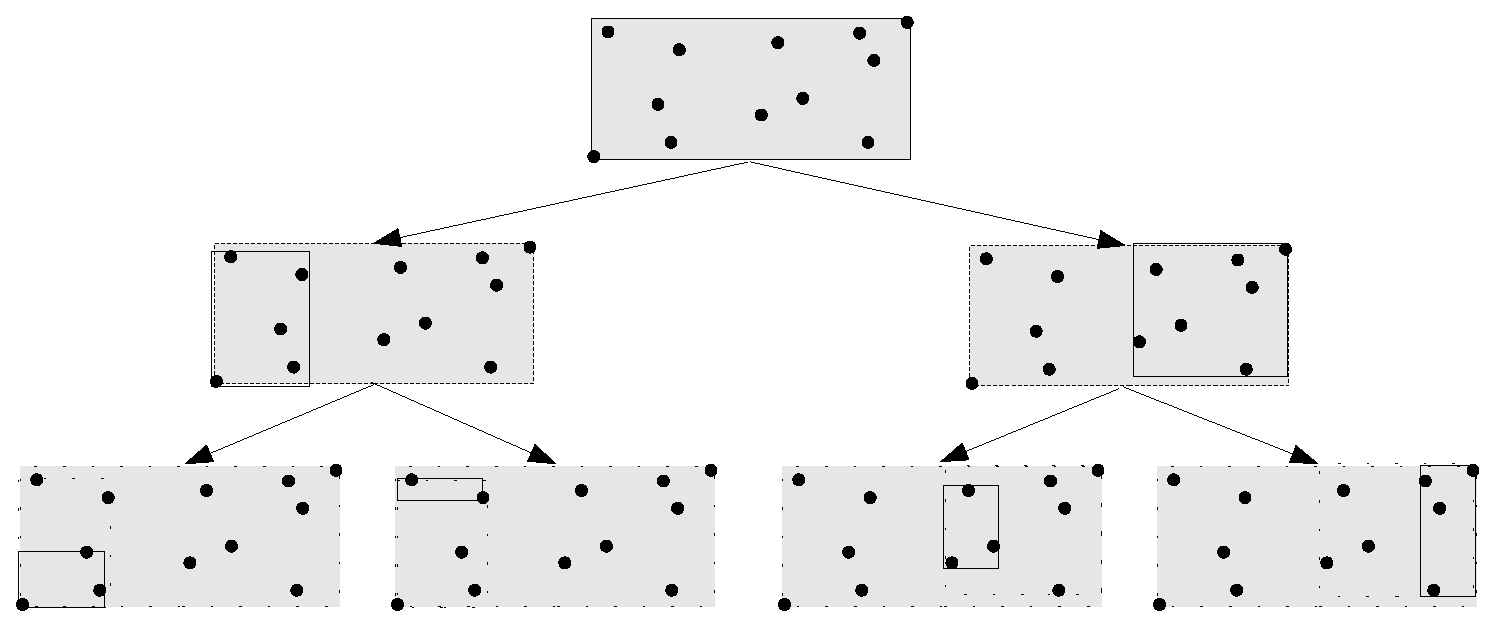
\includegraphics[height=6cm]{kdtree.eps}}
\caption{A two dimensional kd-tree}
\end{figure}

%\insfig[kdtree]{kdtree.eps}{A two dimensional kd-tree}{8cm}

\begin{figure}[!htb]
\label{dualkdtree}
\centerline{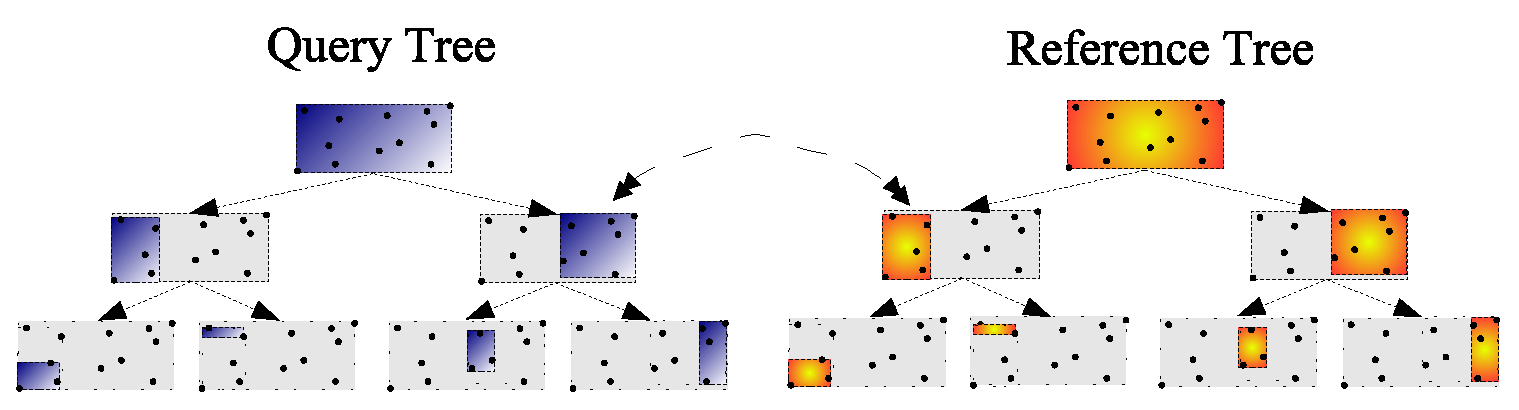
\includegraphics[height=4cm]{dualtree_recursion.eps}}
\caption{Simulation of the dual tree algorithm}
\end{figure}

%\insfig[dualkdtree]{dualtree_recursion.eps}{Simulation of the dual
%tree algorithm}{8cm}

\subsection{Large scale trees, for out of core memory}
\label{Large_scale_trees}

Kd-trees have been proven to be quite successful in
multidimensional indexing and outperform several other
trees in statistical processing of data, mainly in the all nearest
neighbor problem, n-point correlation etc. In this section we
address different implementations of kd-trees for data that don't
fit in the RAM. We show whether virtual memory behaves better   than
paging of nodes on the disk.

Kd-trees have been used quite successfully in statistics for
speeding up statistical algorithms (nearest neighbor, 2 point
correlation) over large datasets \cite{gray2000nbp}. Many other trees like ball trees,
vantage trees, cover trees etc \cite{samet2005fma} have been developed as rivals but
they haven't really shown any significant improvement, their
performance is most of the times comparable to the kd-trees. After
30 years they still remain the state of the art for developing
statistical algorithms. In most of the cases kd trees have been used
for datasets that fit in the main memory.

During the same period the database community developed structures
for multidimensional indexing mainly used for database applications.
Some examples of successful tree structures are R-trees,
$R^{*}$-trees, X-trees and TV-trees \cite{samet2005fma}. The main incentive for these
trees was to handle large volumes of data, dynamic insertions,
deletions and random accesses.

The size of the datasets for statistical processing is increasing
faster than the availability of  main memory so it is necessary to
investigate the performance of kd-trees and various optimizations
over cached implementations. Unfortunately R-tree like structures
cannot be used or even compared to kd-trees since they are optimized
for different problems. It turns out that batch loading of spatial
trees can improve their performance. There are splitting strategies
in some of them (X-trees) that can guarantee non overlapping
hyper-rectangles which is considered to be a good thing for the
nearest neighbor performance. Eventually kd-trees can be considered
as a special case of spatial trees, so there is no point in
comparing them.

In this section we consider some caching implementation strategies for
kd-trees. The first approach is the use of virtual memory through
memory mapped files. The basic advantage is the the programming
simplicity, since data can be accessed through normal pointers. The
operating system takes care of the page faults. The second approach
is to take care of the cache so that we can use bigger page sizes
than the default 4096 in Linux. Page fault is handled on the
application level. In order to minimize the io cost between disk and
main memory we used the TPIE library that does efficient block
transfers.

Another parameter that affects the performance of the trees is the
layout of the tree on the memory, that has to be in such a way that
it guarantees good locality in terms of the access pattern of some
basic kd-tree algorithms, such as all  nearest neighbors, n-point
correlation. There are different ways to build a kd-tree: a)Depth
first b)Breadth first and c)The combination of them building k-depth
trees breadth first. It has been shown experimentally that
unbalanced kd-trees tend to give better pruning performance, we also
consider balanced tree splits since they can give better locality.

The last implementational issue is prefetching.  Queries in
databases are random most of the time so prefetching doesn't really
make sense. On the other hand statistical algorithms on trees
generate queries that are highly correlated, so we can take
advantage of that. Taking advantage of the multicore architecture it
is possible to do non blocking system call for prefetching.

We do not address the problem of building cache
efficiently trees since this issue has been extensively addressed in
the literature, with the most successful algorithm the buffer tree
\cite{arge2003btt}.

\subsubsection{Memory layout of Kd-trees} There are many ways to
build a kd-tree, depth first, breadth first and the combination for
both. It turns out that breadth first does not give good locality
for dual-tree algorithms. Another parameter of
kd-trees that has effect in the cache performance is the splitting
algorithm. Mid-point splits  guarantee balanced trees, but do not
always give good performance in terms of punning.

\subsubsection{System architecture} There are several ways to
implement a disk kd-tree. As it has been stated above, speed is an
essential feature that we are particularly interested as well as
portability. Since building the tree for large scale data might take
a lot of time it is very important to be able to reload the tree and
perform other operations. Although it is desirable to keep the tree
as generic as possible so that we can use it for different
applications this might sacrifice the performance. In our
implementation we avoided virtual functions, structures that require
memory reallocations. In order to keep it generic we used simple
concepts of C++ template programming. Another issue that is of great
importance is memory locality. There are five basic memory
structures involved in a kd-tree, nodes, leafs, data points node
cached statistics and hyper-rectangles. Some of them can be combined
but it is always good to preserve the abstraction hierarchy Tree,
Node, bounding Box, Node Statistics, and Points. There is also
another one which can be treated separately, the result. This can be
the nearest neighbor(s), the kernel density estimation etc. They can
be stored either on the tree or on external structures linked from
the tree nodes. There are two major ways to lay out the tree on the
memory. The first method is to use a separate cache for each data
structure and the other one is to use  a single cache for
everything. In some cases the output of the algorithm might as well
be orders of magnitude larger than the actual tree. For example
k/range nearest neighbors can give pretty big result sets for large
k or range.

\subsubsection{Memory Manager Architecture} In order to test
different memory manager strategies, we used smart pointers that
would collaborate with their corresponding memory allocators. Memory
Allocators implement a set of basic functions such as
{\verb"malloc" }.
One of the fundamental issues is to make sure the allocated memory for each
structure had the correct alignment. It is widely known that wrong
memory alignment can decrease the performance or even cause a
program crash. an easy and portable way to compute the memory
alignment is to use the simple macro depicted in \ref{Alignment}. Another issue
that has to be addressed is page fault handling. In the following
section we describe two different memory managers we implemented and
we compare their performance.

\begin{figure}[!htb]
\label{Alignment}
\begin{boxedminipage}[c]{\linewidth}
\begin{verbatim}
template <typename T>
   struct Tchar {
       T t;
       char c;
   } ;
   #define strideof(T)                             \
      ((sizeof(Tchar<T>) > sizeof(T)) ?            \
        sizeof(Tchar<T>)-sizeof(T) : sizeof(T))
\end{verbatim}
\end{boxedminipage}
\caption{Computing the alignment of a struct}
\end{figure}

\paragraph{Memory Mapped Files} In this approach we used a single memory
mapped file big enough to fit the tree. The length of the file has
to be known in advance, but it is not hard to estimate it. The memory is
allocated linearly and since there are no reallocations or deletions
there is no need to worry about memory fragmentation. Paging is
taken care by the operating system. The page size is fixed 4096B for
Linux. Customizing the page size is something desirable but this
shouldn't be of great worry since very soon Linux will accommodate
for variable page size \cite{winwood2002mps}. This implementation is pretty simple and
memory access is achieved with normal pointers. It is also efficient
since all the paging is done in lower levels of the operating system

\paragraph{User defined cache, with TPIE} In this implementation a block of
memory is pre-allocated and page faults are handled in an LRU sense,
while the block transfers between main memory and the disk are done
with the TPIE engine. TPIE is a portable library for efficient block
transfers. It 's highly abstracted to accommodate for different
transfer models. It is currently implementing memory mapped mode,
Linux read/write and C fread/fwrite. In the future it will implement
the parallel disk model as well. The advantage of this memory
manager is that we can control/define several features, such as page
size, page replacement algorithm and disk/memory transfers. The main
disadvantage is the address translation that has to be done on the
application level and slows down the system. In order to minimize
this effect we sacrificed a little bit of the programming interface
simplicity. So the address translation is explicitly done in the
initialization of the pointer. So the pointer includes a universal
address (integer) and a pointer to the main memory. Upon request the
internal pointer p points to the data in the main memory. As it is
obvious this particular memory segment might be paged out during the
execution. To avoid that the programmer explicitly locks the
particular page as long as the pointer is in use and then it is
explicitly unlocked when the data pointing to is not necessary
anymore. This policy is always prone to deadlocks if the cache
size is small and the page size is large. Another possible case of
deadlock is when the tree building algorithm does not guarantee good
locality in the access pattern of the dual-tree algorithm. In
practice we never came across a deadlock, since depth first and
kdepth first give good enough locality for N-body algorithms. But
even in the case of bad locality we could make local copies of the
data and not lock the pages, sacrificing the performance of the
algorithm. It turns out though that the locking/unlocking strategy
is quite efficient because it avoids copies and it minimizes the
cost of address translation. This coding scheme is sensitive to bugs
because the programmer might accidently keep pages locked, which can
have an immediate effect in the program performance in the same way
memory leaks behave. For this reason we trace locks/unlocks in debug
mode to ensure that the program is free of this type of bugs.
Another important issue is marking the modified pages so that we
save unnecessary copies from main memory to disk. We used the
SIGSEGV library along with mprotect to address efficiently this.
Pages are write protected in memory and if a write occurs a signal
is raised and the page is marked as modified.

\subsubsection{Results}
We ran several experiments on a 1GByte Ram machine with data that where  at least twice the
size of the cache (The system would not give more than 700MB to the running process). 
In reality the memory requirements are much larger since there is other overhead stored on the
tree. The results are also stored as key-value pairs. for example: <point id, minimum distance>.
The size of memory requirements depends also on the k-parameter of k-nearest neighbors.
We tested two different strategies, 
\begin{enumerate}
  \item Keep a separate memory mapped output file for the 
        results. Every leaf points to this file, it needs to keep a list with the current candidate
        nearest neighbors. Eventually when the algorithm is done, all the results are stores
        on the external file. The results are shown in table \ref{on_a_separate_file}.
  \item Store the results on the leafs and when the algorithm is done visit the leafs and
        dump them on a file, table \ref{on_the_leaf}
\end{enumerate}
At this point we would like to stress that the range nearest neighbor problem is much more
easy in the implementation. Once a point is within the range it can immediately stored on the
disk, while in the the k-nearest search we know the true k-neighbors after the end of the
whole dual-tree algorithm.

The results state that keeping the results on a separate file breaks the good locality
behavior of the dual-tree algorithm, giving almost double execution time. The profiling
reports show almost 40\% less CPU utilization time because of the frequent page faults.

In table \ref{mmanager_comparison} we see the performance
of the custom made memory manager, with variable page size. The performance is almost 50\%
worse than the memory mapped files. Profiling reports showed that a great overhead is spent
on the memory translation.   

\begin{table}[!htb]
\label{on_a_separate_file}
\footnotesize{ \centering
\begin{tabular}{|c|c|c|c|}
  \hline
  % after \\: \hline or \cline{col1-col2} \cline{col3-col4} ...
  number of points & dimensions & dual-tree time(sec)& initialization (sec)\\
  140000000        & 2          & 2711               & 1730\\
  100000000        & 3          & 4885               & 1338\\
  5000000          & 5          & 8376               & 650\\
  \hline
\end{tabular}
\caption{Cache performance for storing results in separate space. Memory mapped files}
}
\end{table}

\begin{table}[!htb]
\label{on_the_leaf}
\footnotesize{ \centering
\begin{tabular}{|c|c|c|c|}
  \hline
  % after \\: \hline or \cline{col1-col2} \cline{col3-col4} ...
  number of points & dimensions & dual-tree time(sec) & collection (sec)\\
  140000000 & 2 & 2039 & 836\\
  100000000 & 3 & 2648 & 711\\
  5000000   & 5 & 4131 & 430\\
  \hline
\end{tabular}
\caption{Performance for cache that stores everything on the tree. Memory mapped files}
}
\end{table}

\begin{table}[!htb]
\label{mmanager_comparison}
\footnotesize{ \centering
\begin{tabular}{|c|c|c|c|c|}
  \hline
   number of points & dimension & page size & dual-tree(sec) & collection(sec) \\
   140000000 & 2 & 65536   & 25432 & 2482 \\
   140000000 & 2 & 524288  & 4978  & 2026 \\
   140000000 & 2 & 1048576 & 4438  & 1901 \\
   140000000 & 2 & 4194304 & 4543  & 1819 \\
   100000000 & 3 & 65536   & 8163  & 1603 \\
   100000000 & 3 & 524288  & 6542  & 1499 \\
   100000000 & 3 & 1048576 & 6094  & 1386 \\
   100000000 & 3 & 4194304 & 6618  & 1283 \\
 \hline
\end{tabular}
\caption{Cache performance for different page size and different datasets. Custom made cache}
}
\end{table}


\subsection{Kernel methods}
\label{Kernel_methods}

The kernel or Gram matrix is an informational representation
for a set of data. There are  different interpretations for the
kernel matrix. The most mathematical interpretation is the dot
product matrix. Every element of the kernel matrix is the dot
product between two data points. It is a positive semidefinite
matrix and it can be considered as the adjacency matrix of a graph
where the points are nodes. This graph can also be considered as an
approximation of the surface that data lie on. Positive
semidefinitness is the only property required for the gram matrix.
In most of the methods that we discuss in this section, we prefer
the interpretation of the dot product matrix, in the general Hilbert
sense. The dot products in most of the cases are non-linear.

\subsubsection{Kernel principal component analysis}
\label{Kernel_principal_component_analysis}

Kernel Principal Component Analysis (KPCA) \cite{scholkopf2002lks}, is an extension of
principal component analysis where the data are mapped into a
different feature space through the kernel. In Principal Component
Analysis the goal is to find the principal components for  the
covariance matrix $C$ for a given dataset $S=\{x_j, x_j\in \Re^d, j=1
\dots M\}$, where $C=\frac{1}{M}\sum_{j=1}^{M}x_j x_j^T$. We
define a mapping
\begin{equation}
\Phi : x \rightarrow X , x \in \Re^d, X\in \Re^f
\end{equation}
usually $f>>d$. So  the nonlinear mapping, maps the data in a
higher dimensional space sometimes in an infinite dimensional space.
At this point it should be clarified that the mapping increases the
extrinsic dimensionality of the data not the intrinsic. In kernel PCA we
want to find the principal components of the covariance matrix
\begin{equation}
\tilde{C} = \frac{1}{M}\sum_{j=1}^{M}\phi(x_j)\phi(x_j)^T
\end{equation}
It turns out that the mapping $\Phi$ doesn't have to be known
explicitly, all we need is the kernel that represents the dot
product.
\begin{equation}
k(x, y) = \phi(x)\phi(y)^T
\end{equation}
For some kernels there is an analytic factorization while for others
there is not. Not every function can be a valid kernel (dot
product). There are conditions that must be fulfilled. Basically for
every dataset they  must give a valid kernel matrix as described in
previous sections.

Kernel PCA has many cousins such as Laplacian eigenmaps
\cite{Belkin}, Diffusion maps  \cite{Lafon}, Isomap \cite{tenenbaum2000ggf},
Local Linear Embedding \cite{roweis1993ndr},
Local Tangent Space Alignment \cite{zhang2002pma} etc.
%Both works present algorithms for computing the Laplace-Beltrami
%operator on a submanifold $\Gamma$ embedded in $\Re^d$.
Lafon has introduced a diffusion process on the manifold based on a
kernel $k(x,y)$ that defines the local geometry on the points that
belong to the manifold. The choice of the kernel affects essentially
the results of the diffusion process, since it affects the notion of
the neighborhood around the points which is critical for the
creation of the proximity graph of the manifold. In their work
Belkin \cite{Belkin} and Lafon don't deal with the problem of training the local
bandwidth of the kernel, assuming that the manifold has been
sufficiently sampled. Jenssen \cite{jenssen17lpd} has proven  that
there is a theoretical equivalence between the Mercer kernel and the
kernel in kernel density estimation. Based on that fact we performed
several experiments using the optimal bandwidth for kernel density
estimation. The Adaptive Kernel Based Density
Estimation Algorithm (AKDEA) \cite{Silverman} was chosen. The
proposed algorithm is a partial solution because it doesn't deal
with the final objective function directly, which in some
applications of manifold learning it could be clustering or
dimensionality reduction.

The connection between manifold learning and Kernel Density Estimation (KDE) has also been addressed in \cite{girolami2002osd} 
by using
orthogonal series density estimation rather than kernel density
estimation

%In  section 2 the diffusion operator is reviewed based on the work
%of Lafon \cite{Lafon}. Section 3 outlines the adaptive kernel
%estimation algorithm. The last section presents examples of the
%diffusion operator when the kernel bandwidth is trained.

\subsubsection{Geometric diffusion on a manifold}
Let  $(\Gamma,\mu)$
be a measure space, where $\Gamma$ is a finite set of
$d$-dimensional points and $\mu$ is a counting measure that
represents the distribution of the points on the  data set. In other
words $\Gamma$ is a submanifold of $\Re^{d}$. Assume that the
geometry of $\Gamma$ is defined by a kernel $k(x,y)$. The kernel
$k(x,y)$ measures the degree of similarity between two points $x,y$.
The kernel satisfies the following conditions:
\begin{itemize}
    \item   $k$ is symmetric: $k(x,y)=k(y,x)$,
    \item   $k$ is positivity-preserving: for all $x,y$ in
$\Gamma, k(x,y)\geq 0$
    \item   $k$ is positive semi-definite: for all bounded
functions $f$ defined on  $\Gamma$,
\[
\int_{\Gamma} \int_{\Gamma} k(x,y)f(x)f(y)d\mu(x)d\mu(y)\geq 0\]
\end{itemize}
It is assumed that $\Gamma$ is a subset of the
Euclidean space $\Re^{d}$. So for $x,y\in\Gamma$ the kernel
(similarity measure) is a function of the Euclidean distance
$\parallel x-y\parallel:$
\[
 k(x,y)=\eta\left(\frac{\parallel x-y\parallel}{h}\right)
\]
In order to study the geometry of the submanifold $\Gamma$, an
oriented graph $G$ is formed. Every node corresponds to a data
point. Let $b(x,y)$ be the associated adjacency matrix, where
$b(x,y)=1$ if $x$ is in the neighborhood of $y$ and $b(x,y)=0$ if
$x$ is not in the neighborhood of $y$. The kernel $k$ defines the
notion of neighborhood between the points.

Let $u^2(x)=\int_{\Gamma}k(x,y)d\mu(y)$, then the normalized kernel
$a(x,y)=\frac{k(x,y)}{u(x)u(y)}$ is stochastic since:
\begin{equation}\label{kernel}
    \int_{\Gamma}a(x,y)d\mu(y)=1.
\end{equation}

The kernel $a(x,y)$ can be considered as a transition matrix of a
Markov process on the submanifold $\Gamma$. So any admissible kernel
can be associated with a random walk on $\Gamma$. The operator
\[
    Af(x)=\int_{\Gamma}a(x,y)f(y)d\mu(y)
\]
is called a diffusion operator. The eigenvalue analysis of the graph
with the adjacency matrix $a(x,y)$ is the basis for embedding the
data to a lower dimensional space.
\[
    a(x,y)=\sum_{j=0}^{M} \lambda_{j}\phi_{j}(x)\phi_{j}(y)
\]
where $M$ is the number of data points, $x,y$ are nodes of the graph
and $\phi_j$ is the $j_{th}$ eigenvector of $a$ that corresponds to
the $\lambda_j$ eigenvalue.


%\subsubsection{Kernel PCA on a manifold}
%\label{Kernel_PCA_on_a_manifold}
%
%Let  $(\Gamma,\mu)$ be a measure space, where $\Gamma$ is a finite
%set of $N$-dimensional points and $\mu$ is a counting measure that
%represents the distribution of the points on the data set. In other
%words $\Gamma$ is a submanifold of $\Re^{n}$. Assume that the
%geometry of $\Gamma$ is defined by a kernel $k(x,y)$. The kernel
%$k(x,y)$ measures the degree of similarity between two points $x,y$.
%The kernel satisfies the following conditions:
%\begin{itemize}
%    \item   $k$ is symmetric: $k(x,y)=k(y,x)$,
%    \item   $k$ is positivity-preserving: for all $x,y$ in
%$\Gamma, k(x,y)\geq 0$
%    \item   $k$ is positive semi-definite: for all bounded
%functions $f$ defined on  $\Gamma$,
%\[
%\int_{\Gamma} \int_{\Gamma} k(x,y)f(x)f(y)d\mu(x)d\mu(y)\geq 0\]
%\end{itemize}
%It is assumed that $\Gamma$ is a subset of the Euclidean space
%$\Re^{n}$. So for $x,y\ni\Gamma$ the kernel (similarity measure) is
%a function of the Euclidean distance $\parallel x-y\parallel:$
%\[
% k(x,y)=\eta\left(\frac{\parallel x-y\parallel}{h}\right)
%\]
%The eigenvalue analysis of the graph with the adjacency matrix
%$k(x,y)$ is the basis for embedding the data to a lower dimensional
%space.
%\[
%    k(x,y)=\sum_{j=0}^{M} \lambda_{j}\phi_{j}(x)\phi_{j}(y)
%\]
%
%where $M$ is the number of data points, $x$ and $y$ are nodes of the
%graph and $\phi_j$ is the $jth$ eigenvector that corresponds to the
%$\lambda_j$ eigenvalue.
%
%One problem is that exhaustive computation of the kernel will lead
%to a full matrix, which makes the computation of the eigenvector
%$O(N^2)$. Fortunately very few $(x,y)$ pairs have a non zero kernel
%product since it depends on their proximity. So again the
%computational bottleneck for kernel PCA is the computation of
%nearest neighbors which can be solved by the dual tree algorithm in
%linear time.

\subsection{Parameter estimation for manifold learning, through density estimation}
\label{Bandwidth_Tuning}
Manifold learning turns out to be a very useful tool for many
applications of machine learning, such as classification.
Unfortunately the existing algorithms use ad hoc selection of the
parameters that define the geometry of the manifold. The parameter
choice affects significantly the performance of manifold learning
algorithms. Recent theoretical work has proven the equivalence
between the Mercer kernel learning methods and the kernel in kernel
density estimation. Based on this fact the problem of kernel
parameter estimation for manifold learning is addressed based on the
nonparametric statistical theory estimation. An automatic way of
determining the local bandwidths that define the geometry is
introduced. The results show that the automatic bandwidth selection
leads to improved clustering performance and reduces the
computational load versus ad hoc selection.

\subsubsection{Non parametric  density estimation} The problem of
density estimation of finite data set is very significant for most
of the well known machine learning algorithms. Lafon has proven that
the Laplace Beltrami operator on a manifold can be computed without
the knowledge of the density. Although the density is not necessary
for the computation of the operator it can be useful in the
estimation of the parameters of the kernel eq.~\ref{kernel}.

The  density estimate $f$ of a finite set of data $X={x_i\ni
\Re^n,i=1,\dots,M}$ can be expressed with the following equation
\cite{Silverman}:
\begin{equation}\label{powerdensity}
    f(x)=\frac{1}{M}\sum_{i=1}^{M}\frac{1}{h^d}k\left(\frac{\parallel x-x_i
\parallel}{h}\right)
\end{equation}
The shape of the density function varies significantly with
different values of $h$, which is the global bandwidth. Higher
values of $h$ lead to smoothed versions of the  density. An
automatic way to determine the optimum value of $h$ is to maximize
the Leave One Out Cross Validation (LOOCV) criterion. In other words
the density is formed according to (\ref{powerdensity}) by leaving
one point out and then the probability of this point is evaluated
according to the density. The LOOCV can be mathematically expressed:
\begin{equation}
    M(h)=\sum_{i=1}^{M}\log\sum_{i\neq j}f_j(x_i)
\end{equation}
where $f_j$ is the density computed according to
(\ref{powerdensity}) by leaving $x_j$ out.

Another restriction that can be imposed to the estimated density is
the minimization of the power of the second derivative of the
density $\int f''(x)^2$. This restriction tends to give smoother
densities and avoids the formation of isolated islands of points.
With the standard optimization techniques $h$ can be chosen.

The value of $h$ defines the neighborhood around a point through the
kernel $k$. For dense areas $h$ has to be small, while in sparse
areas $h$ must be high since the points are far away from each
other. This leads to the conclusion that $h$ should be different for
every point. The density can be written in the form:
\[
    f(x)=\frac{1}{M}\sum_{i=1}^{M}\frac{1}{(\lambda_i h)^d}k(\frac{\parallel x-x_i
\parallel}{\lambda_i h})
\]
The $\lambda_i$ are called local bandwidths. The local bandwidths
can be estimated from the following algorithm:
\begin{itemize}
    \item Find a pilot estimate $\tilde{f}(x)$ that satisfies
         $\tilde{f(x_i)>0, i=1,\dots,M}$
    \item The local bandwidth $\lambda_i$ is given by:
        \[
            \lambda_i=(\tilde{f}(x_i)/g)^{\frac{1}{d}}
        \]
        where g is the geometric mean  of the $\tilde{f}(x_i)$:
        \[
            g=\sqrt[M]{\prod_{i=1}^{M}\tilde{f}(x_i)}
        \]
    \item The adaptive kernel estimate $f(x)$ is defined by:
         \[
            f(x)=\frac{1}{M}\sum_{i=1}^{M}\frac{1}{(\lambda_i
            h)^d} k\left( \frac{\parallel x-x_i \parallel}{\lambda_i h} \right)
        \]
\end{itemize}
The pilot estimate can be any ad hoc density estimate. A common
estimate is the \emph{kth  nearest neighbor estimate} defined by:
    \[
        \tilde{f}(x)=\frac{1}{Md_k(x)}\sum_{i=1}^{M}k\left(\frac{
        \parallel x-x_i \parallel}{d_k(x)}\right)
    \]
where $d_k(x)$ is the distance between $x$ and the $kth$ nearest
neighbor. It turns out that the choice of $k$ doesn't affect the
values of $\lambda_i$. The adaptive kernel estimate can be improved
if we iterate the above procedure by replacing in every iteration
the pilot density estimate with the adaptive kernel estimate
computed in the last step.
\subsubsection{Eigenvalue analysis of the diffusion graph}
In the previous section we saw that the
non-parametric estimation can  define the local bandwidth for every
point. This information can be used in the construction of the
adjacency matrix $G$. The local bandwidths as derived from the
previous section will usually give a graph that has connected
components, or equivalently the manifold is connected. A  safe test
to prove that is to look into the eigenvalues also known as the
spectrum of the graph. According to \cite{Cvetkovic} the
multiplicity of the first eigenvalue reflects the number of
disconnected components in the graph. There are cases where the
local bandwidths might not give a connected manifold, then it is
necessary to increase $h$ until the multiplicity of the first
eigenvalue becomes 1.

\subsubsection{Kernel choice} There are many classes of kernels that
can be used for the diffusion operator on the manifold. The most
popular is the Gaussian kernel:
\[
    k(x)=\frac{1}{(2\pi)^{-\frac{d}{2}}}e^{-\frac{1}{2}xx^T}
\]

The problem with the gaussian kernel is that it is of infinite
support and it leads to adjacency matrices that are not sparse. It
would be preferable to use a kernel of finite support. The most
popular one is the Epanechnikov kernel \cite{Silverman}:
\begin{equation}
    k(x)=\left\{
    \begin{array}{ll}
        \frac{1}{2}c_{d}^{-1}(d+2)(1-x^Tx) &  x^Tx<1 \\
        0   &   x^Tx\geq 1 \\
    \end{array}
 \right.
\end{equation}

\subsubsection{Examples} In this section two examples illustrated in
the two dimensional space are presented and a third one on real
speech data. The first example fig.~\ref{fig1} contains two clusters
of data. Each cluster contains 300 points uniformly distributed in a
unity area square. The Average Nearest Neighbor Distance (ANND) as a
choice for the bandwidth for the Epanechnikov kernel turns out to be
inadequate since it leads to a disconnected graph with 4 disjoint
components. This is probably because the two classes are sparsely
sampled. The AKDE based on maximization of LOOCV gives on the
average local bandwidths that are an order of magnitude higher than
the ANND, and lead to a smoother density. As it is shown in
fig.~\ref{fig1}b the density is not flat as it was expected to be
and this is because of the fact that the number of points that
sample the manifold is small. In fig.~\ref{fig1}c the first non
trivial eigenvector is depicted discriminating very sharply the two
classes. In fig.~\ref{fig1.1} the same data set is analyzed with a
higher global bandwidth. The results are very poor since there is
high intra-class deviation and the centroids of the two classes are
closer.

The second example fig.~\ref{fig2} illustrates two classes of data
that lie on two halves of a circle, slightly separated. The clusters
are highly the sampled around the angle  of $90^0$ degrees. This
fact makes very difficult to chose a universal value for the local
bandwidths since the notion of the locality is significantly
different in different areas of the manifold. In fig.~\ref{fig2}b
the  density of the data points is shown, reflecting the high
concentration of points around the angle of $90^0$. In this case the
AKDE trains the local bandwidths $\lambda_i$ and the global $h$, so
that the LOOCV is maximized. The resulting values give a manifold
graph that is disconnected in two classes. A  slight increase in the
global bandwidth makes the graph connected.  The first non-trivial
eigenvector of the diffusion operator identifies very clearly the
two classes as shown in fig.~\ref{fig2}c. If the global bandwidth is
increased by an order of magnitude, then still the first non-trivial
eigenvector identifies the two classes, but the classes are not
compact and their centroids are closer fig.\ref{fig3}c. Another
disadvantage of keeping $h$ large is that the adjacency matrix
$a(x,y)$ fig.~\ref{fig5}b of the manifold graph becomes dense. This
increases tremendously the memory requirement and the computation of
the eigenvectors.

In this third example the effect of the local bandwidth on the
clustering problem of three phoneme classes is presented. The points
correspond to the Fast Fourier Transform of 20 msec speech frames
sampled at 8KHz, of the TIMIT database. 200 points from the three
phoneme classes /aa/,/ih/,/sh/ where chosen. In fig.~\ref{fig4}a the
data are plotted in 2 dimensions after the dimensionality reduction
process. It is clear that the diffusion process separates the
classes very well. In fig.~\ref{fig4}b where the bandwidth is an
order of magnitude larger than the optimal, the diffusion process
still separates the  classes, but the clusters are not very compact.
When the local bandwidth is an order of magnitude smaller than the
optimal, the results are very poor. The corresponding graph
fig.~\ref{fig5}c shows that the points are isolated and not
connected.




\subsubsection{Discussion} In this section the problem of constructing
the diffusion graph of a manifold defined by data points in $\Re^d$
was addressed. The parameters of the kernel that define the geometry
over the manifold were automatically trained through the estimation
of the adaptive kernel based density  algorithm. Experiments on
synthetic and real data showed that  if the global bandwidth is
smaller than the one that maximizes the LOOCV, then the graph that
represents the manifold is disconnected into  many spurious
clusters. On the other hand if the bandwidth is higher, then the
diffusion operator will still identify the clusters, but their
distance is smaller and they are not as compact compared to the
optimal bandwidth. Moreover high bandwidth lead to dense graphs and
as a consequence more computations.

The approach followed is still  heuristic, although it has  an
underlying theoretical justification on the work described at
\cite{jenssen17lpd}. It is the first time that experimental results
are presented that show the effect of optimal kernel density
estimation on the manifold learning.

%\instbfig[fig1.1]{fig1.1b.eps}{fig1.1c.eps}{The same data with
%fig.~\ref{fig1}a analyzed with a  larger global bandwidth. (a) The
%estimated density, (b) The first non-trivial
%eigenvector}{4.5cm}{4.5cm}

\begin{figure}[!htb]
  \centerline{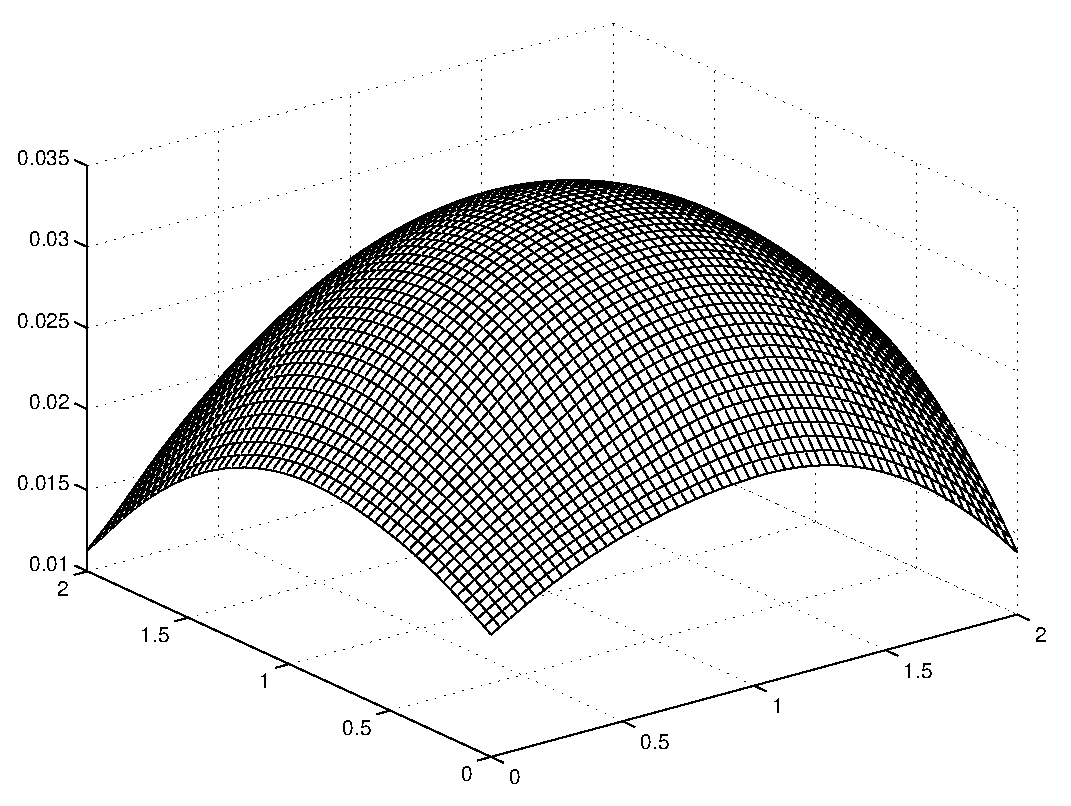
\includegraphics[height=4.5cm]{fig1.1b.eps}(a)}
  \centerline{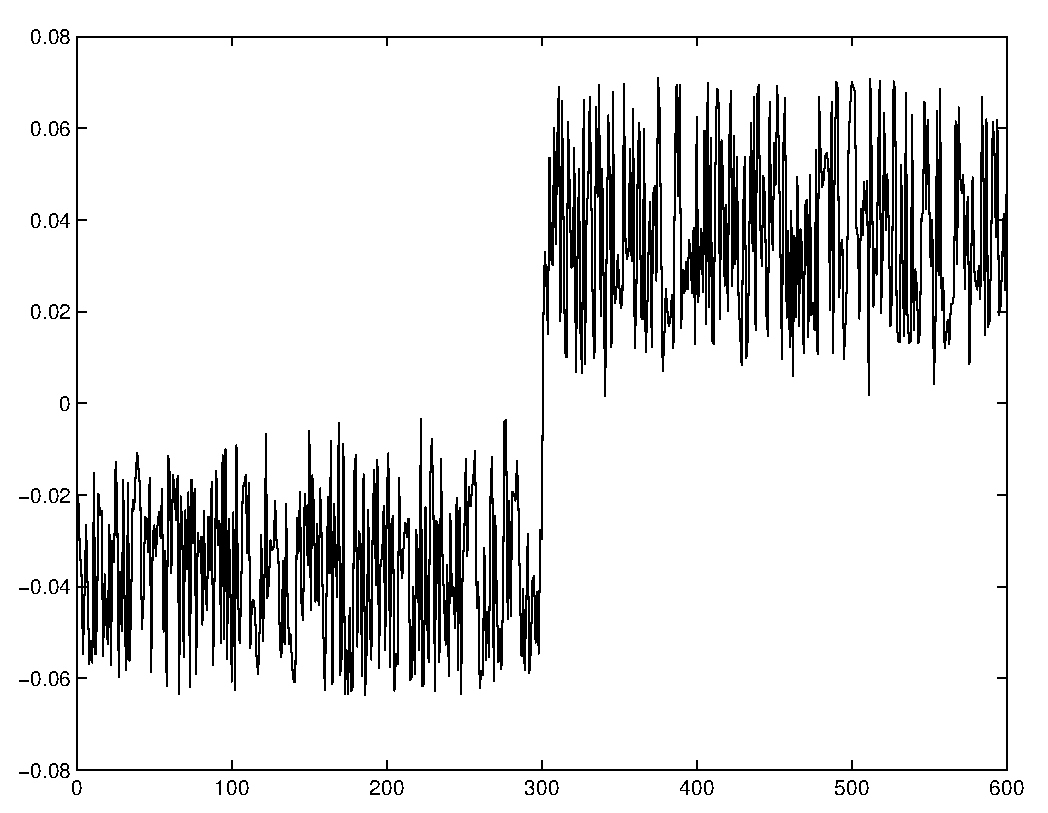
\includegraphics[height=4.5cm]{fig1.1c.eps}(b)}
  \caption{The same data with fig.~\ref{fig1}a analyzed with a
  larger global bandwidth. (a) The estimated density, (b) The first
  non-trivial eigenvector }
  \label{fig1.1}
\end{figure}

%\inssssfig[fig1]{fig1a.eps}{fig1b.eps}{fig1c.eps}{(a) Two clusters
%of uniformly distributed 2-D points, (b) The estimated density, (c)
%The first non-trivial eigenvector}{4.5cm}{4.5cm}{4.5cm}

\begin{figure}[!htb]
 \centerline{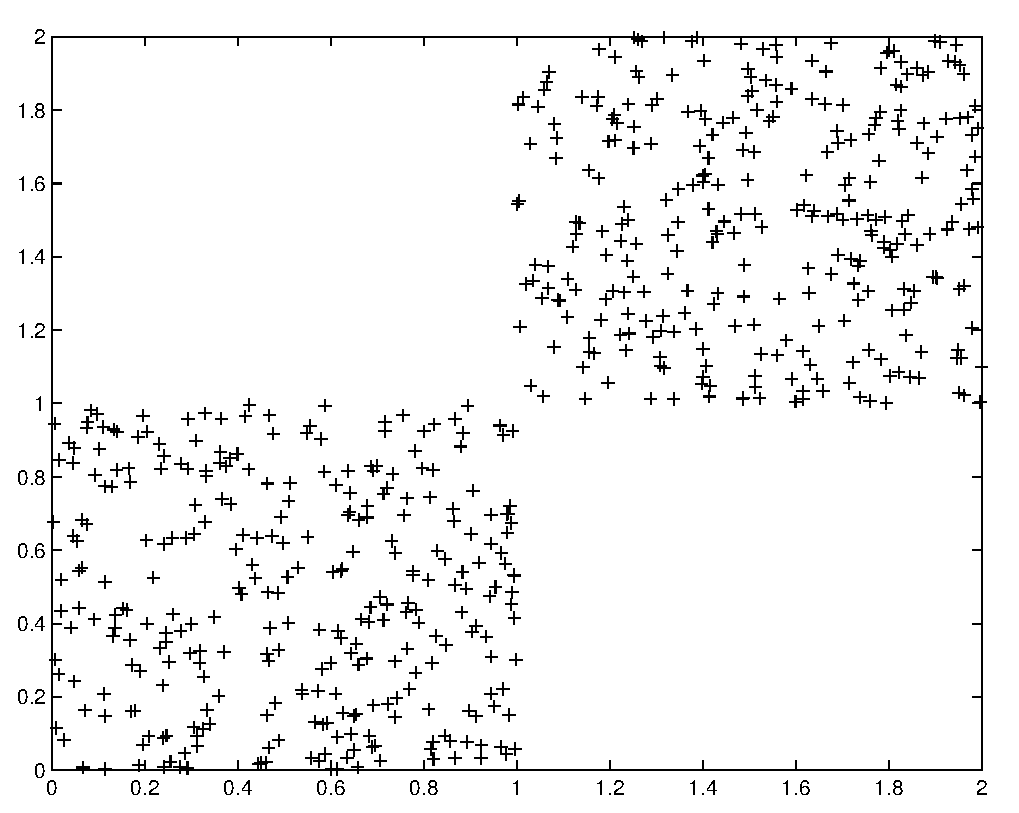
\includegraphics[height=4.4cm]{fig1a.eps}(a)}
 \centerline{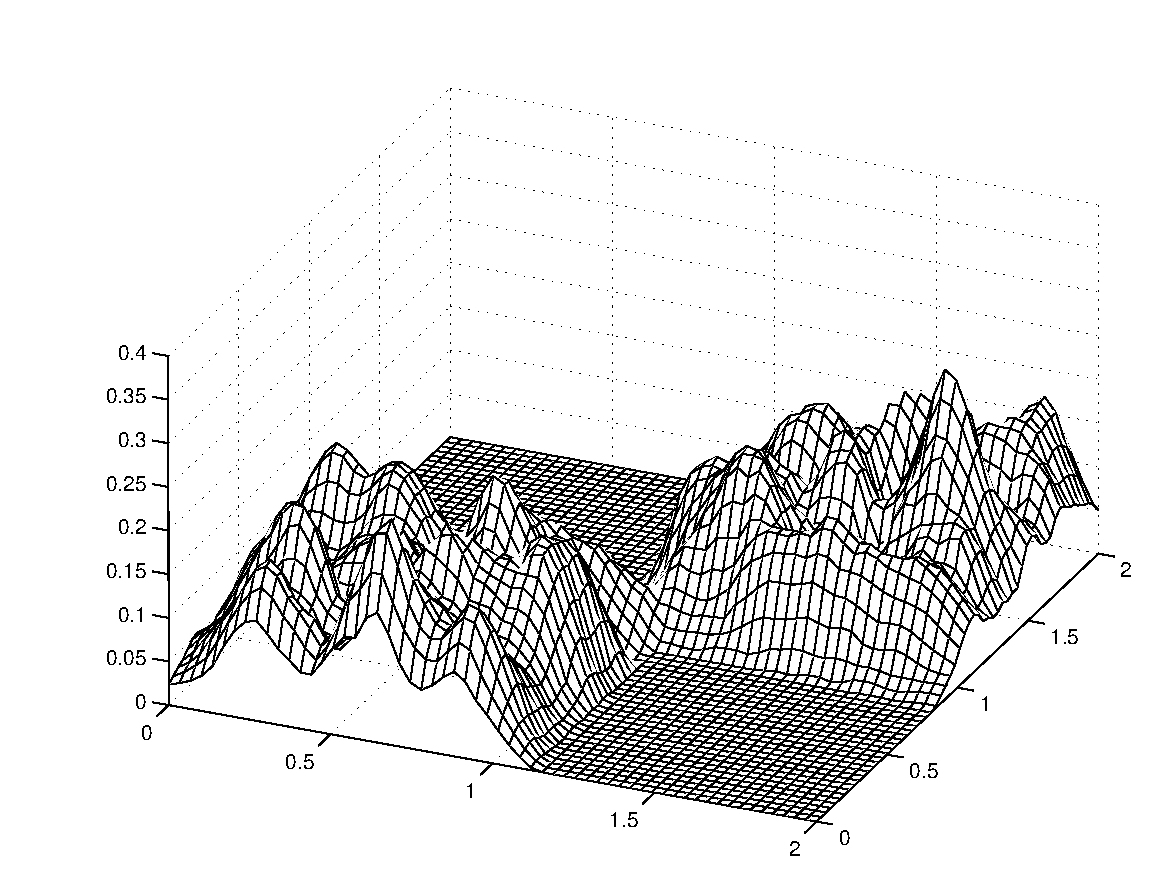
\includegraphics[height=4.4cm]{fig1b.eps}(b)}
 \centerline{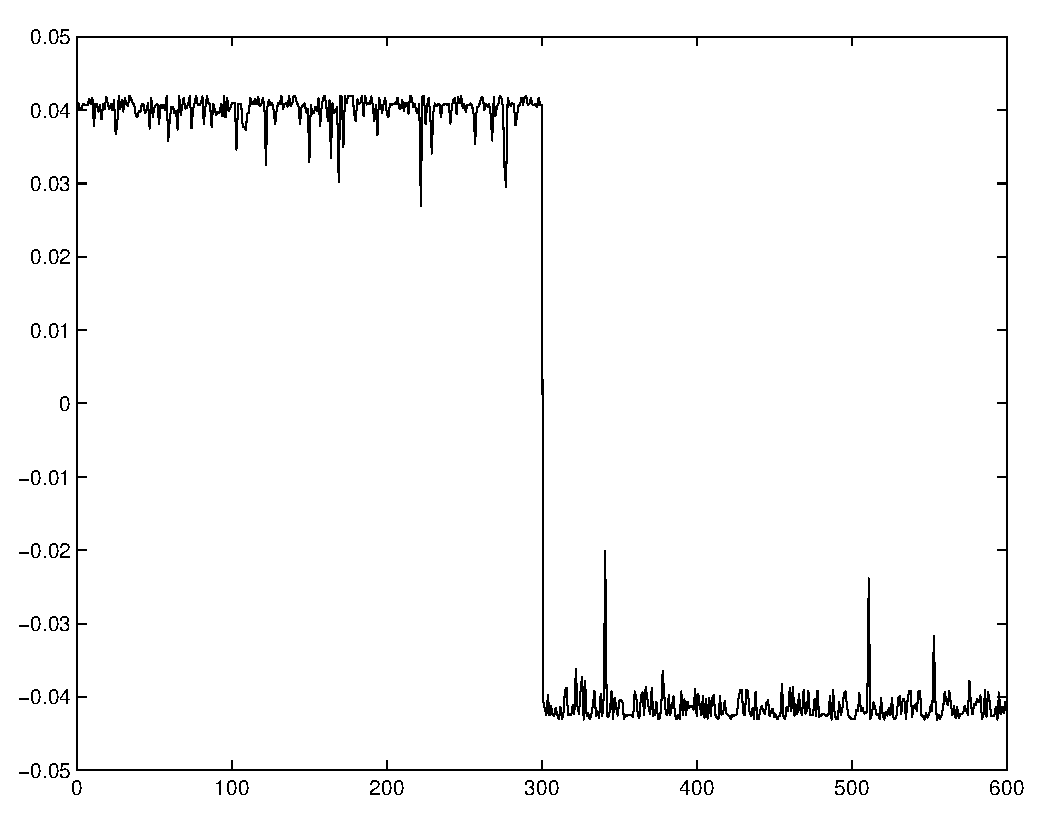
\includegraphics[height=4.4cm]{fig1c.eps}(c)}
 \caption{(a) Two clusters of uniformly distributed 2-D points,
(b) The estimated density, (c) The first non-trivial eigenvector }
  \label{fig1}
\end{figure}

%\inssssfig[fig2]{fig2a.eps}{fig2b.eps}{fig2c.eps}{(a) Two clusters
%of non-uniformly distributed 2-D points, (b)The estimated density,
%(c) The first non-trivial eigenvector}{6cm}{6cm}{6cm}

\begin{figure}[!htb]
 \centerline{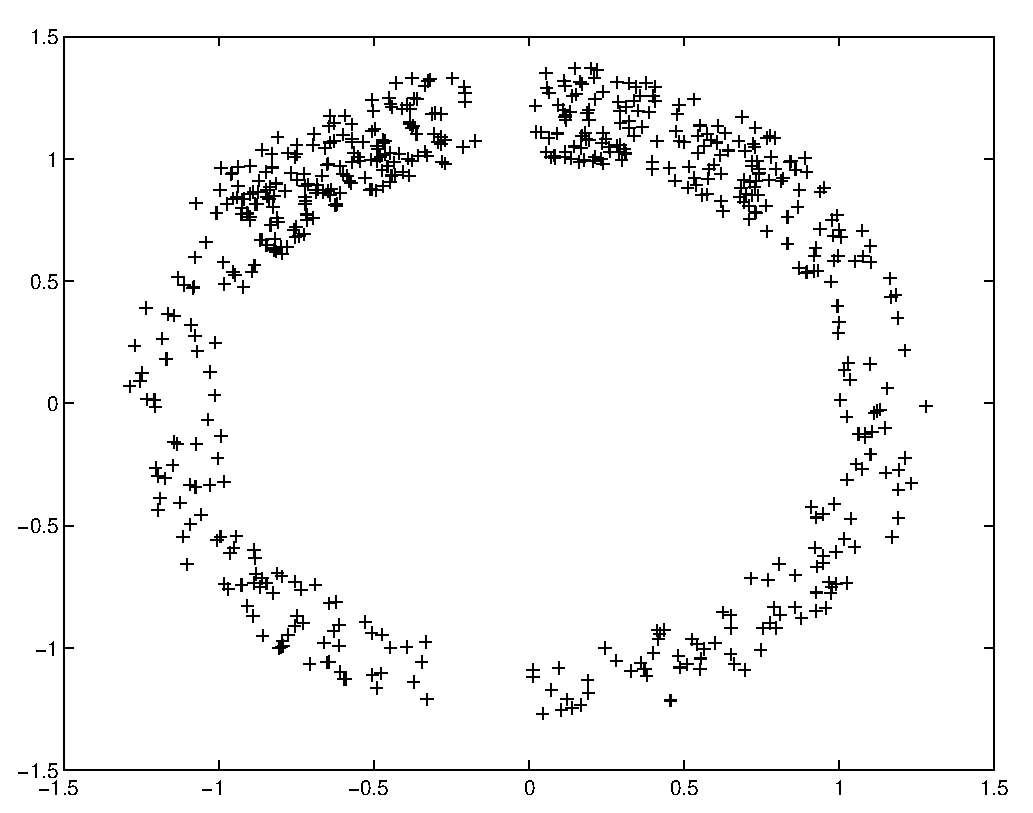
\includegraphics[height=6.0cm]{fig2a.eps}(a)}
 \centerline{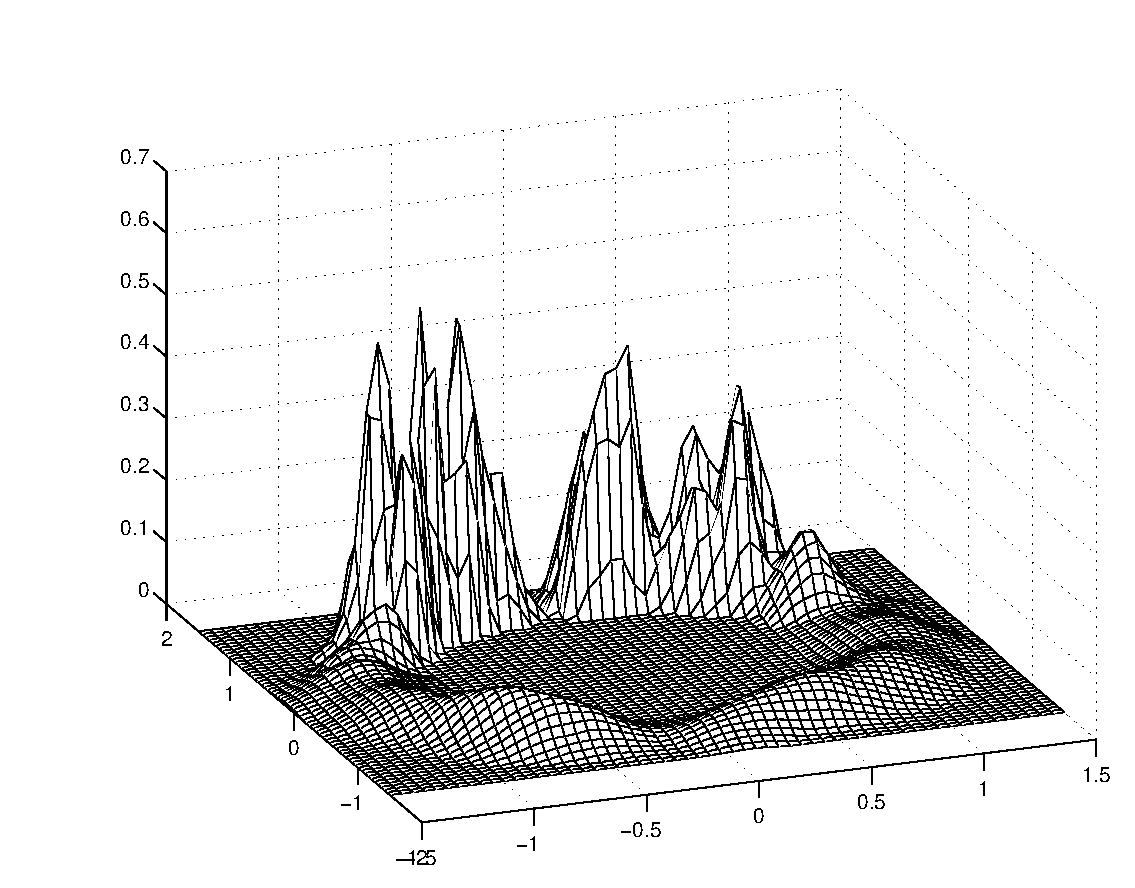
\includegraphics[height=6.0cm]{fig2b.eps}(b)}
 \centerline{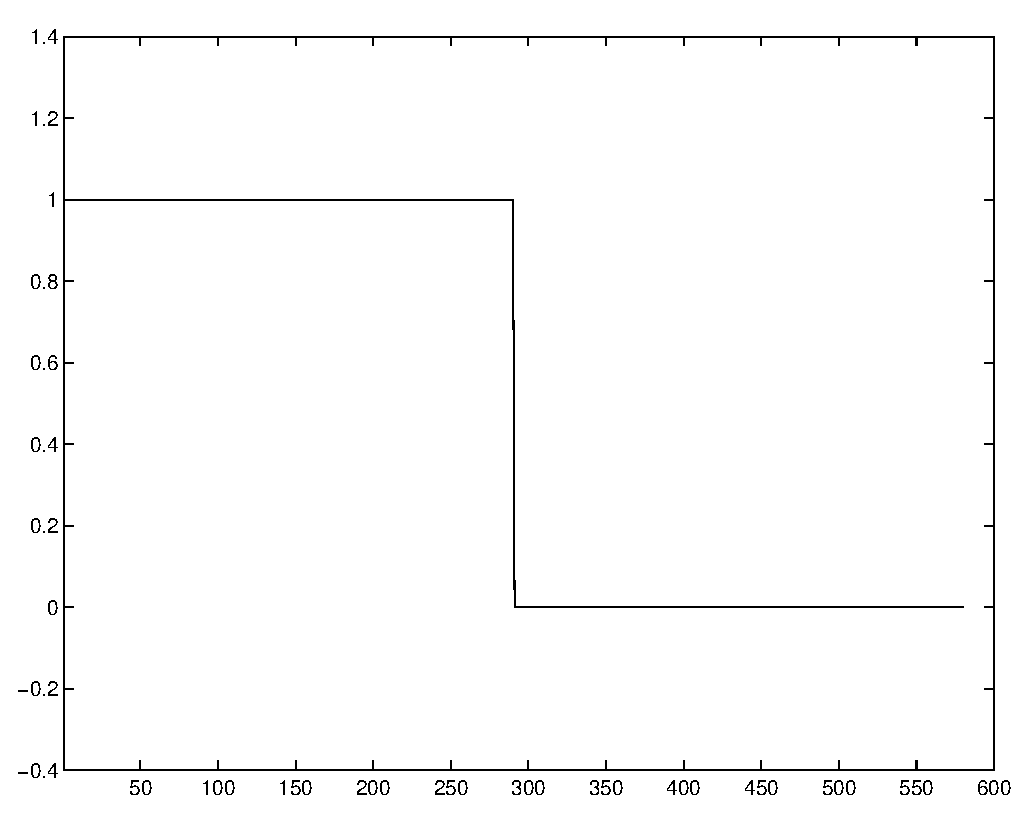
\includegraphics[height=6.0cm]{fig2c.eps}(c)}
\caption{(a) Two clusters of non-uniformly distributed 2-D points,
(b)The estimated density, (c) The first non-trivial eigenvector
\vspace{1.2cm}}
  \label{fig2}
\end{figure}

%\inssssfig[fig3]{fig3a.eps}{fig3b.eps}{fig3c.eps}{The same data set
%with fig.~\ref{fig2} processed with a bandwidth one order of
%magnitude larger. Although the first eigenvector still separates the
%two classes, the classes are closer and not compact (a) Two clusters
%of non-uniformly distributes 2-D points, (b)The estimated density,
%(c) The first non trivial eigenvector}{6cm}{6cm}{6cm}

\begin{figure}[!htb]
 \centerline{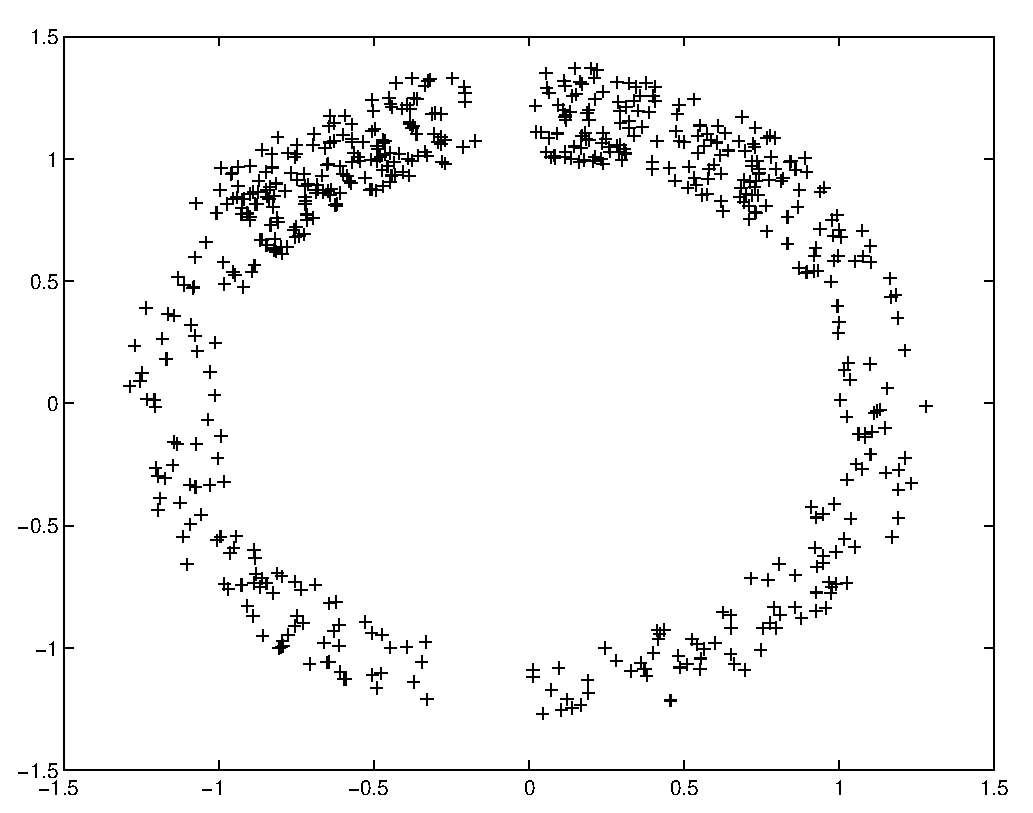
\includegraphics[height=6cm]{fig3a.eps}(a)}
 \centerline{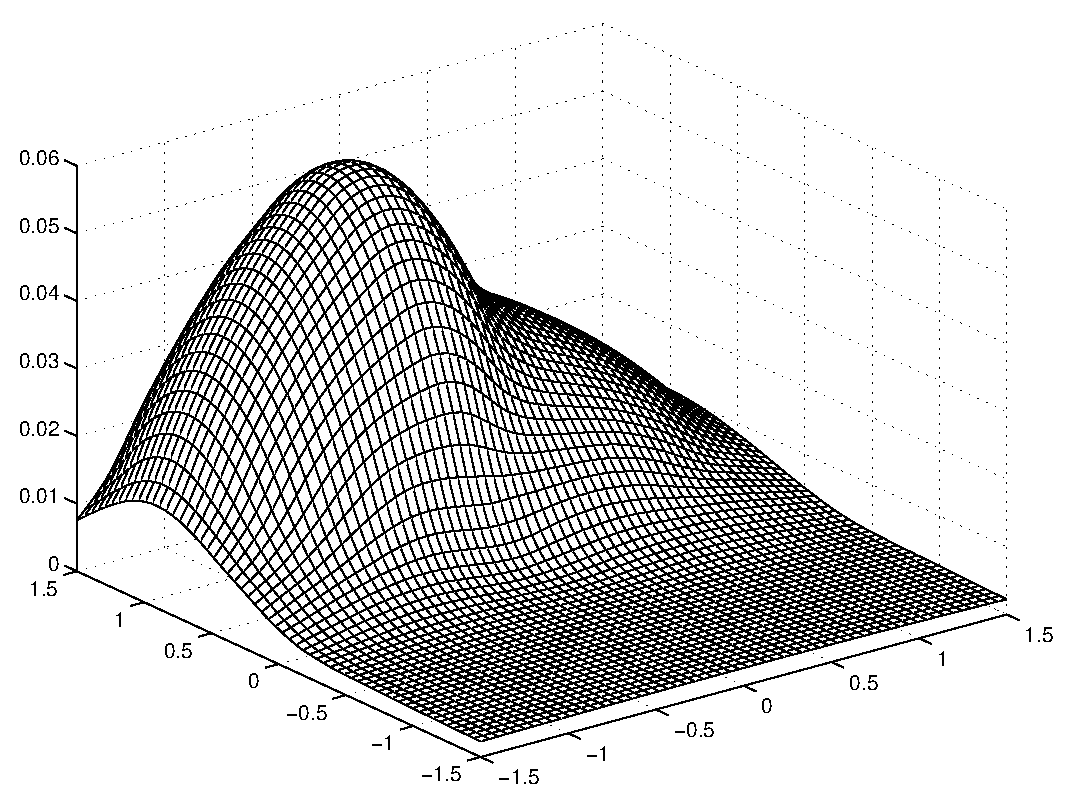
\includegraphics[height=6cm]{fig3b.eps}(b)}
 \centerline{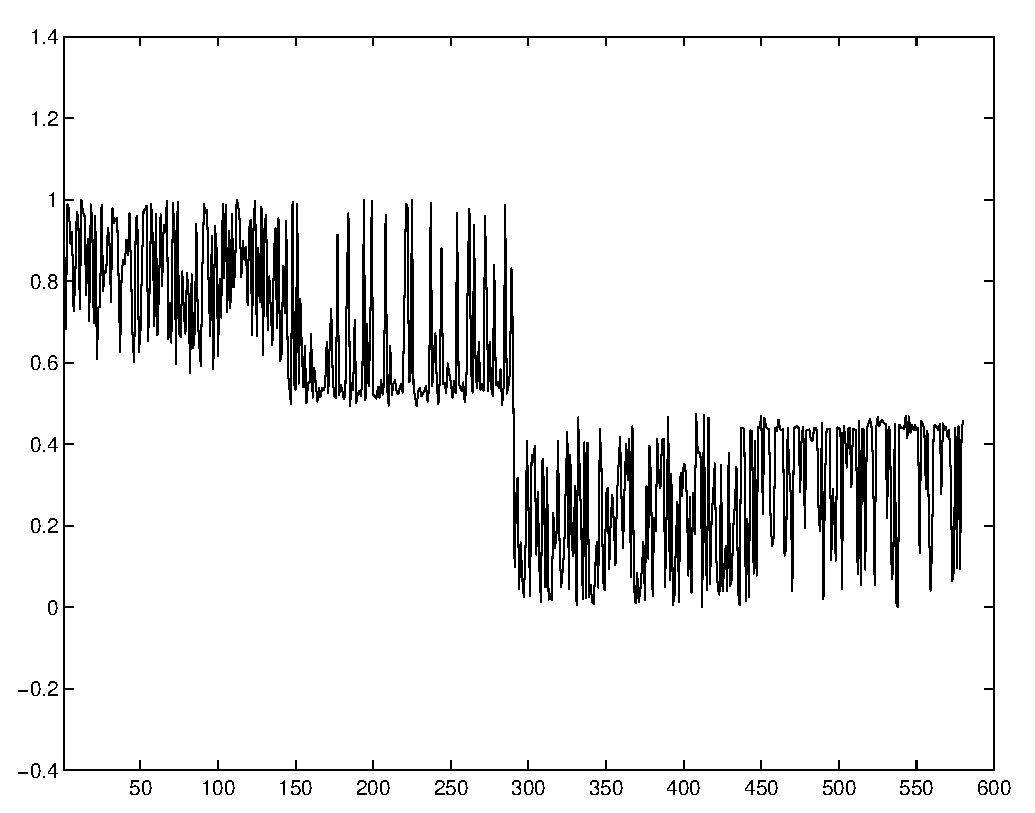
\includegraphics[height=6cm]{fig3c.eps}(c)}
\caption{The same data set with fig.~\ref{fig2} processed with a
bandwidth one order of magnitude larger. Although the first
eigenvector still separates the two classes, the classes are closer
and not compact (a) Two clusters of non-uniformly distributes 2-D
points, (b)The estimated density, (c) The first non trivial
eigenvector }
  \label{fig3}
\end{figure}

%\inssssfig[fig4]{fig4a.eps}{fig4c.eps}{fig4e.eps}{(a) The 3 phoneme
%classes after the dimensionality reduction with the optimal
%bandwidth, plotted in two dimensions, (b) The 3 phoneme classes with
%a larger bandwidth,(c) The 3 phoneme classes with a smaller
%bandwidth}{6cm}{6cm}{6cm}

\begin{figure}[!htb]
 \centerline{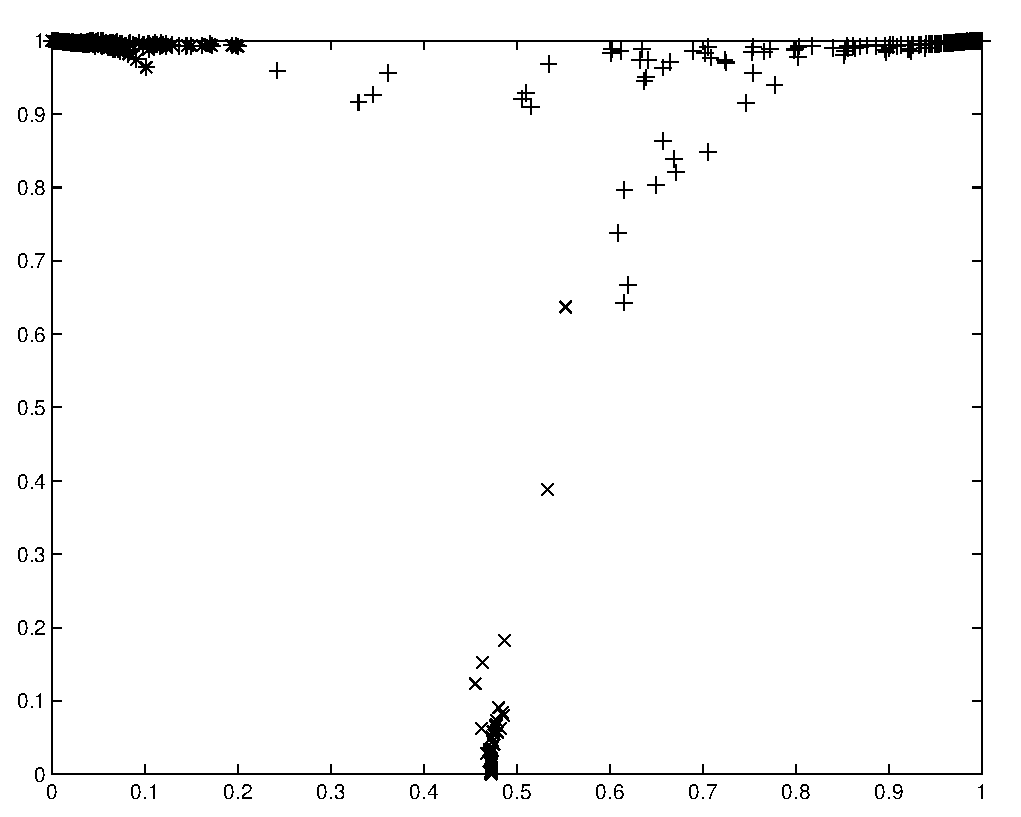
\includegraphics[height=6cm]{fig4a.eps}(a)}
 \centerline{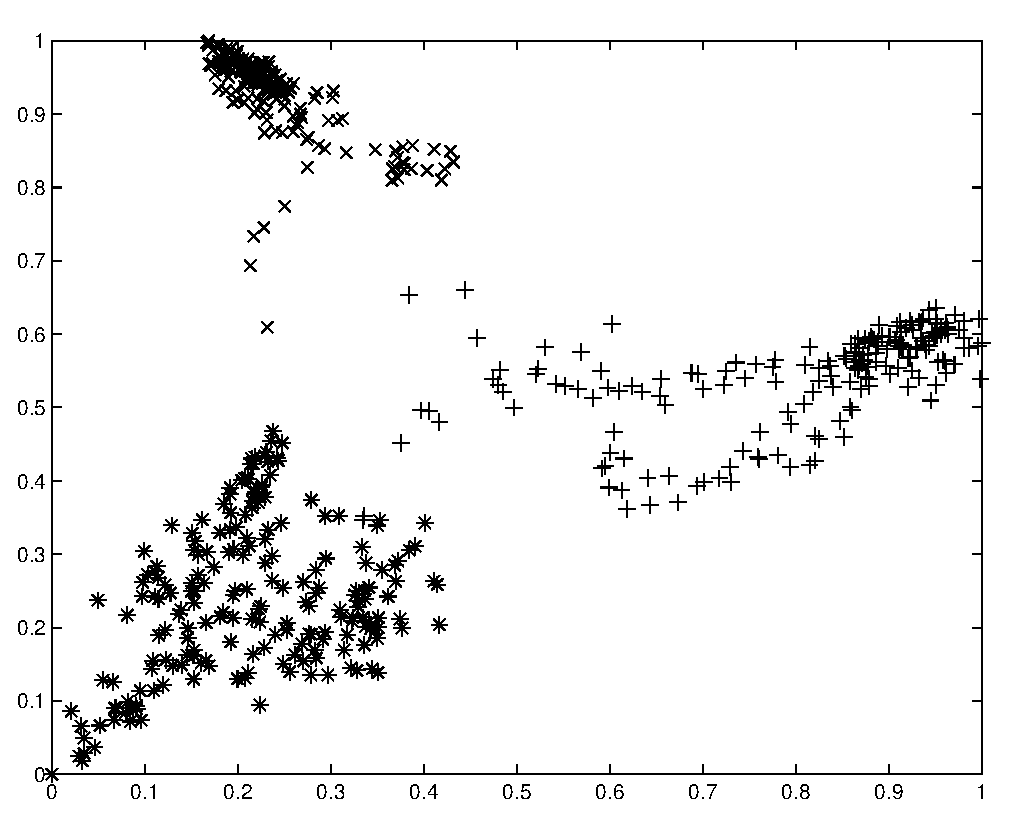
\includegraphics[height=6cm]{fig4c.eps}(b)}
\centerline{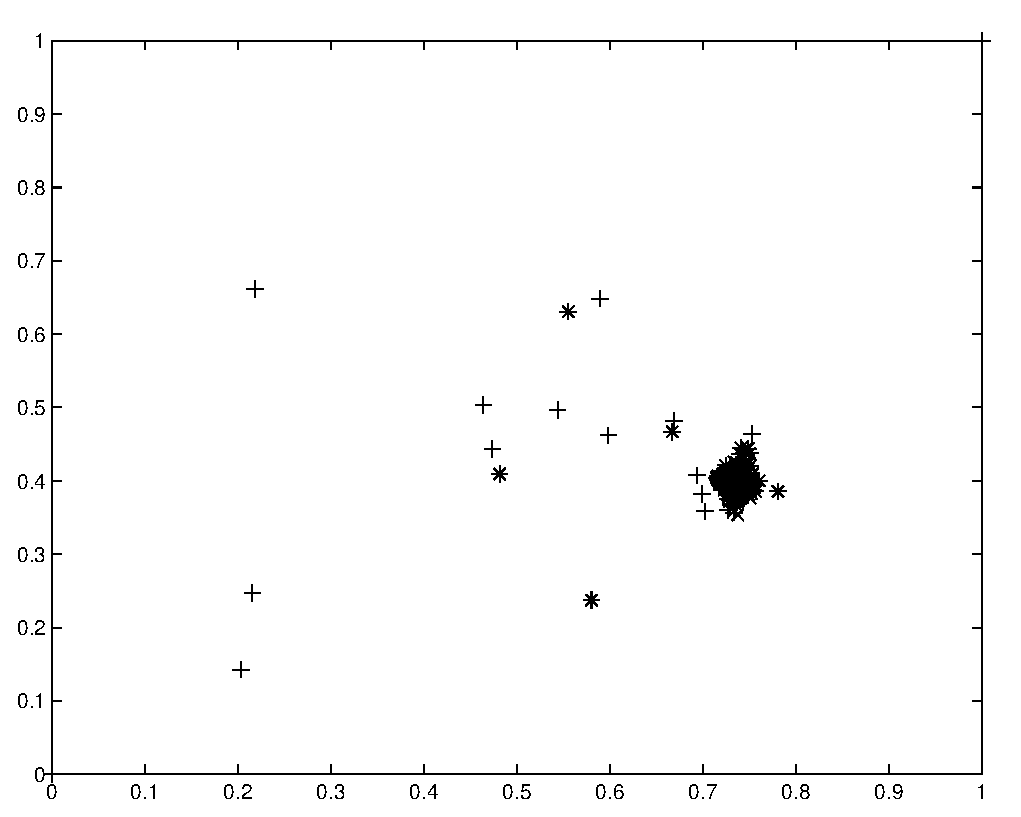
\includegraphics[height=6cm]{fig4e.eps}(c)}
 \caption{(a) The 3 phoneme classes after the dimensionality reduction
with the optimal bandwidth, plotted in two dimensions, (b) The 3
phoneme classes with a larger bandwidth,(c) The 3 phoneme classes
with a smaller bandwidth}
  \label{fig4}
\end{figure}

%\inssssfig[fig5]{fig4b.eps}{fig4d.eps}{fig4f.eps}{The diffusion
%graph for three different local bandwidths (a)Optimal, (b)An order
%of magnitude larger, (c)An order of magnitude
%smaller}{6cm}{6cm}{6cm}

\begin{figure}[!htb]
 \centerline{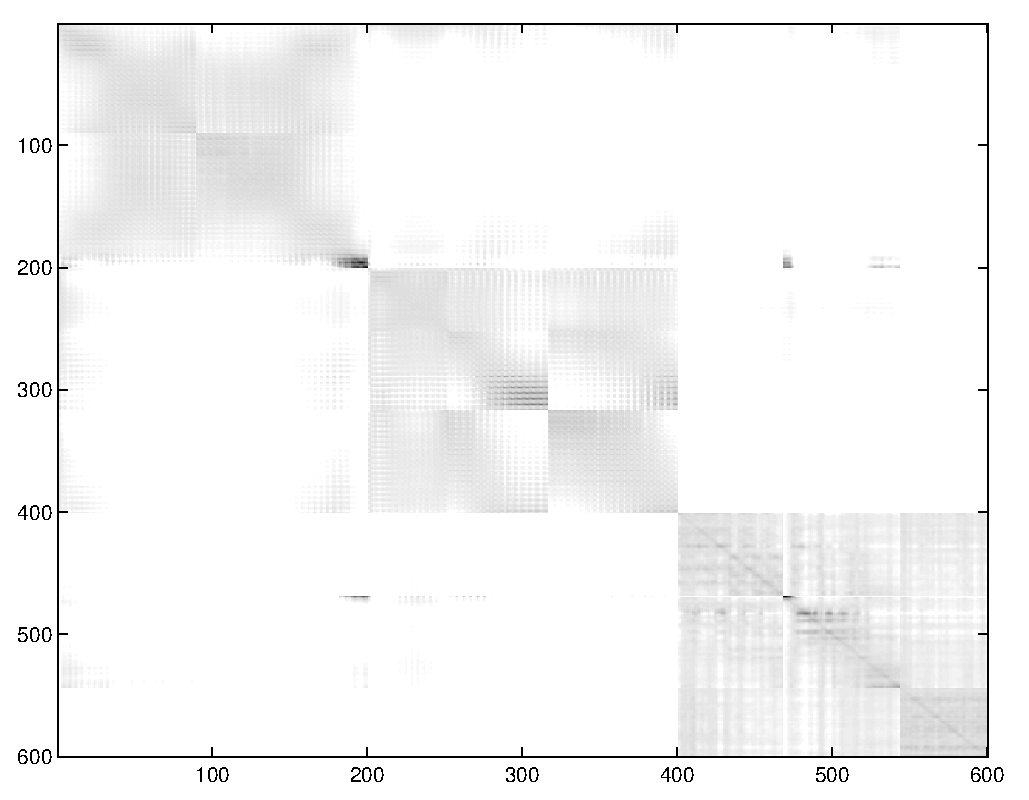
\includegraphics[height=6cm]{fig4b.eps}(a)}
\centerline{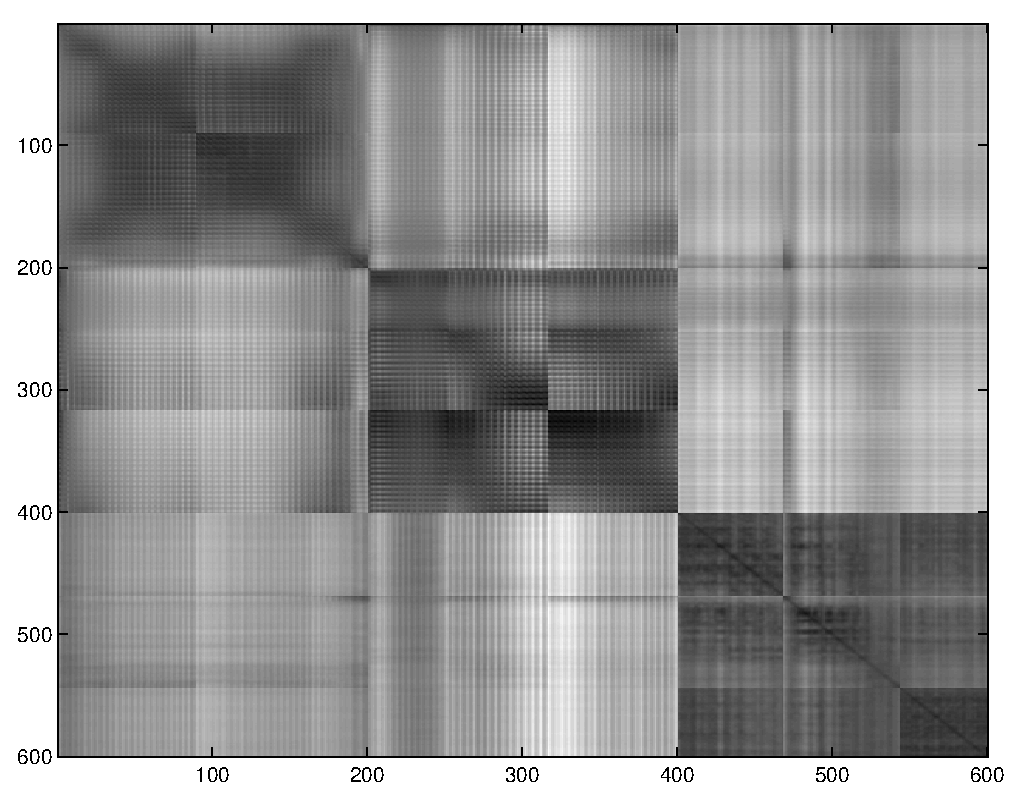
\includegraphics[height=6cm]{fig4d.eps}(b)}
\centerline{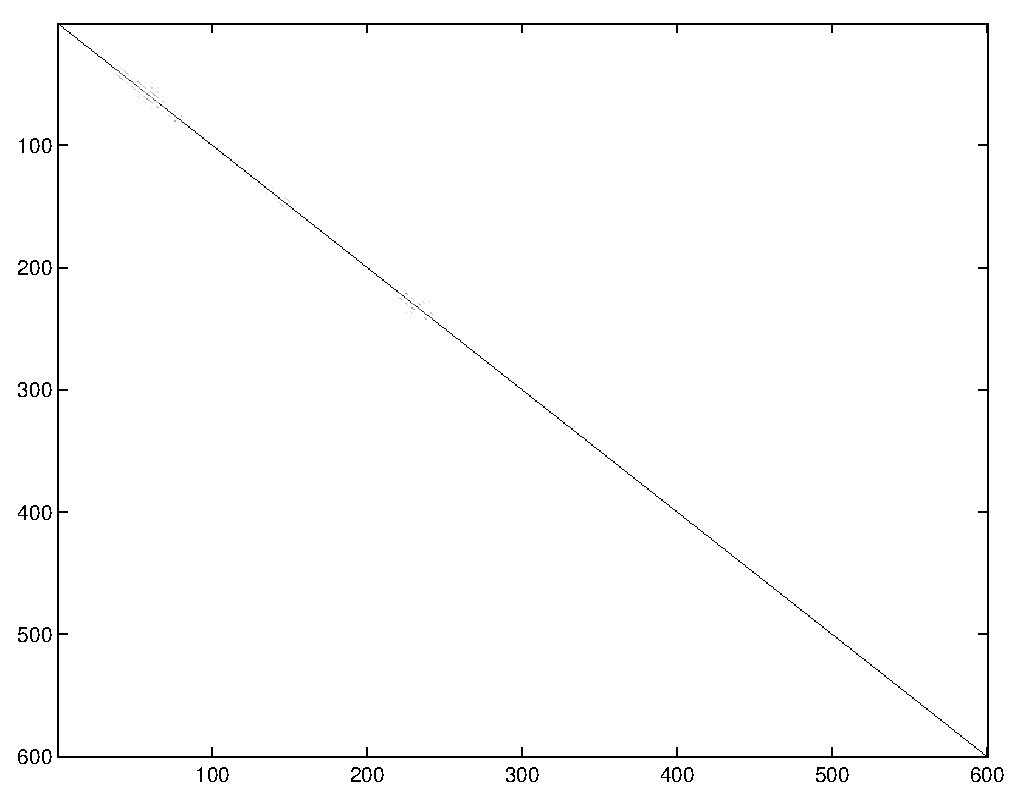
\includegraphics[height=6cm]{fig4f.eps}(c)}
 \caption{The diffusion graph for three different local bandwidths
(a)Optimal, (b)An order of magnitude larger, (c)An order of
magnitude smaller}
  \label{fig5}
\end{figure}


\subsection{Preliminary investigation of nearest neighbor search for speech recognition}

In this section we present a computationally efficient means of
characterizing different features for speech processing tasks. The
presented method can be used to compare the performance of features
free of interference from back-end recognition engines that might be
skewed to favor a particular feature. Understanding the intrinsic
characteristics of features would enable us to make the right choice
of features for a given task.

\subsubsection{Introduction}
Many features have been proposed for speech recognition, with Mel
Frequency Cepstrum Coefficients (MFCC) \cite{quatieri2002dts} being
the most popular. Other features have also been developed claiming
better performance than MFCC in limited tests over different data
sets. The most common metric is the speech recognition word accuracy
over TIMIT or any other data set. Unfortunately most of the speech
recognition systems are specifically tuned for MFCCs and it is
difficult to have objective comparison since systems always tend to
favor them.
%In this section we will introduce statistical algorithms
%that can scale easily for large data sets. One very interesting
%statistical measure for features that can be the basis for many
%machine learning algorithms is all nearest neighbors, which is a
%special case for the general N-body problem. The brute force method
%is of $O(N^2)$  complexity and virtually impossible to scale for
%large data sets. One way to speed up computations is to order the
%features on a multidimensional tree, such as kd or ball tree
%\cite{bentley1975bst}, \cite{moore2000ahu} which provide on the
%average $O(N\log_2N)$ complexity for all nearest neighbor search. A
%faster algorithm using 2 trees has made it possible to compute all
%nearest neighbors in linear time \cite{gray2000nbp}.
In this section
we demonstrate the performance of the fast all nearest neighbor
algorithm over the whole TIMIT database using two different
features, MFCC and Noise Robust Auditory Features (NRAF)
\cite{ravindran:inr}. Since the data are phonetically labeled, the
results are used for evaluating the k-nearest neighbor classifier
performance. This is also a good measure for the compactness and
separability of the phonetic classes for these two features.

Another fundamental problem in speech generation theory is the
estimation of the intrinsic dimensionality of the speech manifold. Recent
theories have proven that although speech is described with high
dimensional representations, it is actually embedded on a low
dimensional subspace \cite{jansen2006ifa}. The most easy but
inaccurate method to estimate the embedding of speech in a low
dimensional space is Principal Component Analysis (PCA), which
suffers from many problems, specially because of the presence of
non-linearities on the data. On the contrary many other methods for
dimensionality reduction have been proposed. These are kernel PCA
\cite{scholkopf:nca}, diffusion maps, Laplacian eigenmaps
\cite{coifman2006dm} etc. All these methods operate on a local level
and require the computation of the nearest (range or k) neighbors of
every point. The brute force and single tree methods have made the
cost prohibitive for large data sets, but the dual tree method makes
possible to evaluate the proximity graph between the points and
apply any of the above mentioned methods.

\subsubsection{Speech features} In our implementation, MFCC features
were extracted using the freely available code from \emph{Voicebox}.
The speech signal was divided into frames of length 25 msec, with 50
\% overlap and 13 MFCC coefficients (including the zeroth
coefficient) where extracted from each frame. Twenty-seven filters
were used to group the frequency bins into critical bands.

The NRAF features were derived from a model of the early auditory
system~\cite{shamma_main}. The input signal was passed through a
bandpass filter bank. We then performed a difference operation
between adjacent frequency channels. This is followed by a half-wave
rectification and a smoothing filter. We compute a discrete cosine
transform (DCT) of the logarithm of the output of the smoothing
filter to obtain the NRAFs. The filter bank consisted of 27
1/4$^{th}$ octave filters tuned from 76 Hz to 6887 Hz. The smoothing
(temporal integration) was done over 25 msec and sampled at a rate
of 80 Hz (in order to match MFCCs). As in the case of MFCCs, the
first 13 coefficients were used for further processing.

In both cases the delta and acceleration coefficients were extracted
and appended to each feature vector, increasing the dimensionality
from 13 to 39.

%\subsubsection{Fast N-body methods for feature comparison} One of the
%fundamental problems in statistics is the nearest neighbor
%computation for every point in a dataset. The brute force also known
%as the naive method requires $O(N^2)$ computations. Ordering the
%multidimensional data on a binary tree, gives $O(\log (N)$ search
%time per point and $O(N\log N)$ in total. There is a plethora of
%binary multidimensional trees ball tree, kd tree, cover tree etc. In
%our experiments we used the kd tree. A detailed description of kd
%trees can be found at \cite{moore-tutorial}. The main concept is to
%recursively partition data in disjoint rectangles. Each tree node
%contains a k-dimensional rectangle (hyper rectangle) that bounds all
%the points that are contained in the subtree. Only leafs contain
%points. In Fig.~\ref{kdtree} an example of a kd tree in 2 dimensions
%is given, while the algorithm for computing the nearest neighbor for
%a test point is depicted in table Fig.~\ref{dualtree_algorithm}. The
%main idea is to recursively find the leaf that contains the query
%point then compute a candidate nearest neighbor on the leaf. As the
%algorithm back tracks it determines if it is necessary to search
%other subtrees for a nearest neighbor.
%
%The use of dual trees in the all nearest neighbor search has proven
%to give significant speed-up in all-nearest neighbor computations.
%The basic idea is that the whole query set is structured on a tree.
%In our case the query tree and the reference tree are the same. The
%core of the algorithm relies on the fact that if the current maximum
%nearest neighbor distance in the query node is smaller than the
%distance between the query and the reference node distance then the
%reference node can be pruned. This saves a huge amount of
%computation in most of the cases since whole  subtrees can be pruned
%out for a large subset of points at once. The all nearest neighbor
%search is described algorithmically in Table
%\ref{dualtree_algorithm}. The complexity of the algorithm, on
%average, turns out to be linear.


\subsubsection{Experimental Results} In order to illustrate the
applicability of the algorithms described above, the TIMIT and Noisy
TIMIT (NTIMIT) database were chosen. Our goal is to test our
algorithms in terms of scalability and time. Phoneme classification
with the nearest neighbor classifiers was chosen as the evaluation
task. The task was repeated for both set of features, namely, MFCC
and NRAF. We also illustrate the spectrum of kernel PCA for the two
different features.

\subsubsection{All nearest neighbor performance}
The timing results are illustrated in table \ref{timing}. The all
20-nearest neighbor method with the dual tree algorithm on kd-trees
is 30 to 50 times faster than naive in terms of time. It took about
3.6 hours for MFCCs and 2.2 hours for NRAF for all 20-nearest
neighbors. It is well known that the pruning performance of the
trees depends on the intrinsic dimension of the dataset. A simple
way to get an estimation of the intrinsic dimensionality is the
eigenvalue distribution of the Principal Component Analysis. As seen
from Fig.~\ref{pca} NRAFs have a more compact distribution than
MFCCs.

\subsubsection{Comparison of NRAF and MFCC} 
\label{Feature_Comparison}
Two types of experiments were done for the comparison of the features. The first
one is the Leave One feature Cross Validation. So for every feature
we find the k-nearest neighbors and check whether the majority has
the same label as it \footnote{Instead of using the 61 different
phonetic classes of TIMIT we used the 39 categories of the CMU
dictionary}. In tables \ref{kneighborTIMIT} and
\ref{kneighborNTIMIT}, we demonstrate the performance of MFCC and
NRAF for TIMIT and NTIMIT for various k. NRAF perform better than
MFCC, specially in the noisy case.

In the second experiment we do Leave-One-Speaker-Out cross
validation. For every feature we find the k-nearest neighbors that
don't belong to the same speaker and check if the majority has the
same label as it. The results are illustrated again in
\ref{kneighborLOOCVTIMIT} and \ref{kneighborLOOCVNTIMIT}. The
results drop significantly and it interesting that MFCCs perform
better than NRAFs. The reason why the performance drops
significantly is because we haven't done any covariance
normalization on the data. It is well known in the speech
recognition literature that mean and variance normalization improves
recognition as it removes the speaker bias. It turns out that
variance normalization broadens significantly the PCA spectrum which
is tightly connected with the performance of kd-trees. We tried
variance normalization but the all nearest neighbor performance was
very slow. Another option is the Mahalanobis distance on a metric
tree, but again the covariance normalization would have an immediate
effect on the performance.

It turns out that variance normalization is a way of decorrelating
the MFCC/NRAF dimensions, which breaks the manifold structure. This
is a suggestion that we should move on with higher dimensional
transformations that remove the speaker bias intrinsically.

In fig.~\ref{kernel_pca} the kernel PCA spectrum is illustrated. The
Gaussian kernel with adaptive local bandwidth was used for the
20-nearest neighbors. The bandwidth is proportional to the nearest
neighbor distance and every point is connected with its 20 nearest
neighbors. It turns out that the kernel PCA spectrum is very wide.
This is a result of the fact that 20 nearest neighbors are not
enough to model correctly the manifold. It is an indication that
more neighbors should be used. We experimented with the bandwidths
and it turns out that no further improvement can be achieved by
tuning it. High bandwidths tend to give more compact spectrum, so
even in the extreme case of infinite bandwidth no more significant
improvement is shown for 10 nearest neighbors.

\subsubsection{Discussion} It has been shown previously that NRAFs
tend to be more robust to noise compared to
MFCCs~\cite{ravindran:inr}. From Tables~\ref{kneighborTIMIT}
and~\ref{kneighborNTIMIT} it is clear that NRAFs do provide
substantial improvement over MFCCs specially in noisy environments.
However, it is very interesting to note that MFCCs outperform NRAFs
in all Leave-One-Speaker-Out cross validation tests. This would
suggest that MFCCs are better than NRAFs at removing inter-speaker
variability. Inter-speaker variability usually is the result of
incorporating pitch information (usually encoded in the higher
coefficients of the decorrelation transform) and it is very much
possible that in ensuring NRAFs and MFCCs have the same number of
channels we may have introduced pitch information into the NRAF
features. Perhaps using lesser number of NRAF coefficients or
different filter spacing, the inter-speaker variability could be
removed.

\begin{figure}[!htb]
\label{pca}
\centerline{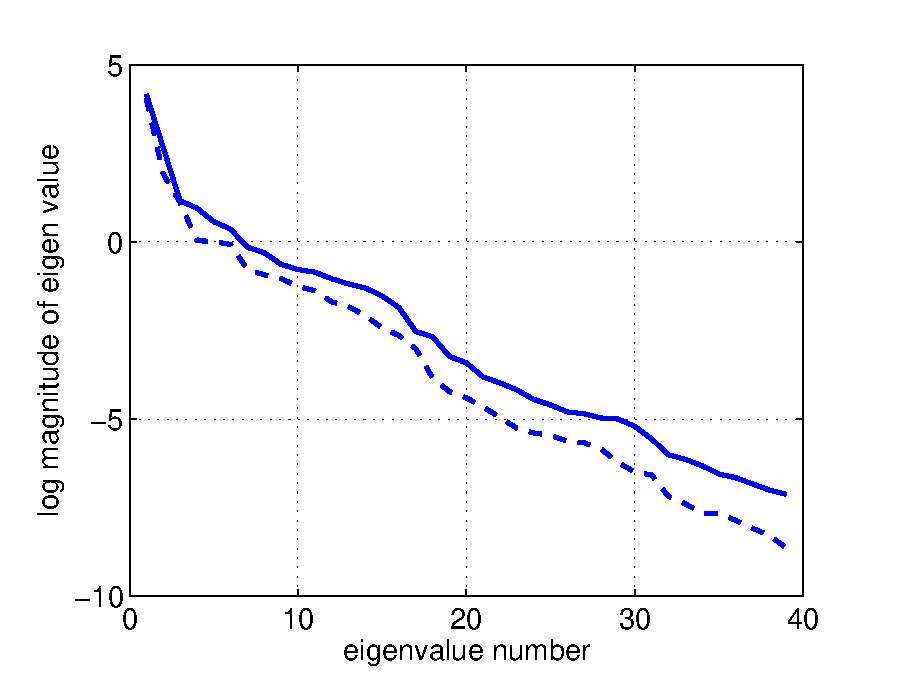
\includegraphics[height=8cm]{timit_pca.eps}}
\centerline{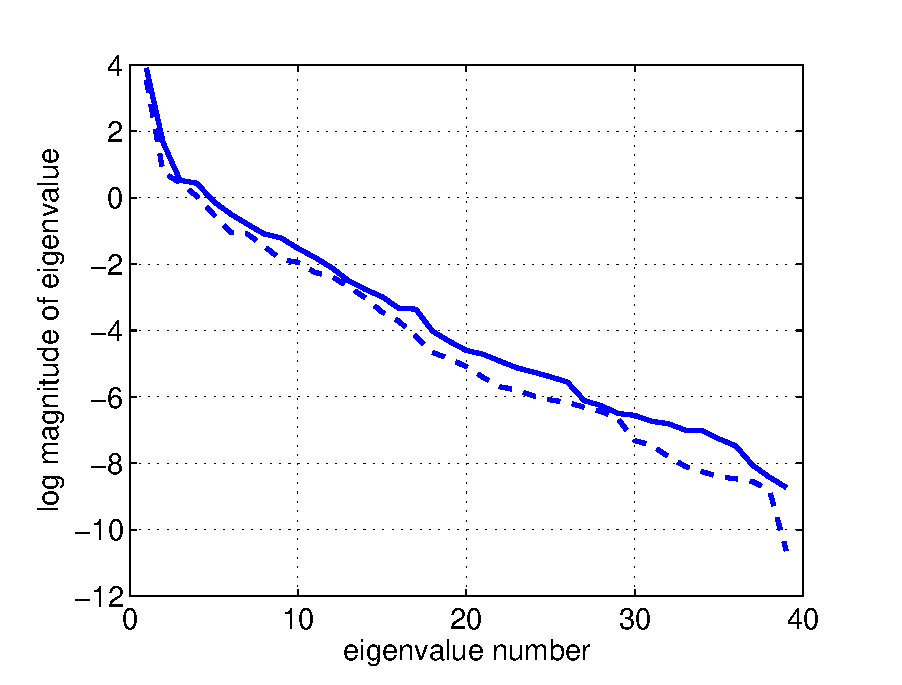
\includegraphics[height=8cm]{ntimit_pca.eps}}
\caption{Principal Component Analysis of TIMIT (top) and NTIMIT (bottom) for MFCC (solid line)
and for NRAF (dashed line).}
\end{figure}

%\instbfig[pca]{timit_pca.eps}{ntimit_pca.eps}{Principal Component
%Analysis of TIMIT (top) and NTIMIT (bottom) for MFCC (solid line)
%and for NRAF (dashed line).}{8cm}{8cm}

\begin{figure}[!htb]
\label{kernel_pca}
\centerline{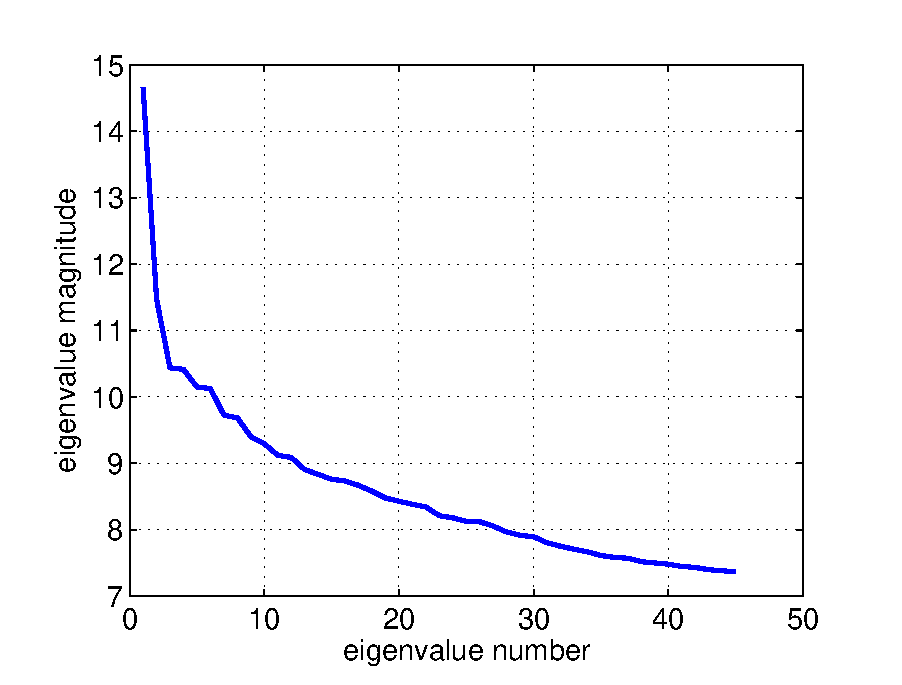
\includegraphics[height=8cm]{kernel_pca.eps}}
\caption{Kernel PCA spectrum for TIMIT MFCC features}
\end{figure}

%\insfig[kernel_pca]{kernel_pca.eps}{Kernel PCA spectrum for TIMIT
%MFCC features}{8cm}

\begin{table}[!htb]
\footnotesize{ \centering
\begin{tabular}{|c|c|c|c|}
  \hline
  % after \\: \hline or \cline{col1-col2} \cline{col3-col4} ...
  feature & Naive & Single Tree & Dual Tree \\
  \hline
  MFCC & 100 & 4.3 & 3.6 \\
  NRAF & 100 & 2.9 & 2.2 \\
  \hline
\end{tabular}
 \caption {CPU time (in hours) for evaluating all 20 nearest neighbors on
  TIMIT database}
  }
  \label{timing}
\end{table}

\begin{table}[!htb]
\footnotesize{ \centering
\begin{tabular}{|c|c|c|c|c|c|}
  \hline
  % after \\: \hline or \cline{col1-col2} \cline{col3-col4} ...
  feature & 1-nearest & 3-nearest & 4-nearest & 7-nearest & 10-nearest \\
  \hline
  MFCC & 62.2\% & 70.4\% & 69.7\% & 65.3\% & 63.4\% \\
  NRAF & 66.9\% & 74.1\% & 73.2\% & 67.3\% & 64.7\% \\
  \hline
\end{tabular}
\caption{Nearest k-neighbor classfier for TIMIT database} }
\label{kneighborTIMIT}
\end{table}

\begin{table}[!htb]
\footnotesize{ \centering
\begin{tabular}{|c|c|c|c|c|c|}
  \hline
  % after \\: \hline or \cline{col1-col2} \cline{col3-col4} ...
  feature & 1-nearest & 3-nearest & 4-nearest & 7-nearest & 10-nearest \\
  \hline
  MFCC & 41.4\% & 55.5\% & 54.5\% & 50.7\% & 49.4\% \\
  NRAF & 55.0\% & 65.1\% & 64.0\% & 57.5\% & 54.5\% \\
  \hline
\end{tabular}
\caption{Nearest k-neighbor classfier for NTIMIT database} }
\label{kneighborNTIMIT}
\end{table}

\begin{table}[!htb]
\footnotesize{ \centering
\begin{tabular}{|c|c|c|c|c|c|}
  \hline
  % after \\: \hline or \cline{col1-col2} \cline{col3-col4} ...
  feature & 1-nearest & 3-nearest & 4-nearest & 7-nearest & 10-nearest \\
  \hline
  MFCC & 44.0\% & 56.3\% & 56.3\% & 54.7\% & 54.6\% \\
  NRAF & 42.2\% & 53.5\% & 53.7\% & 52.4\% & 52.4\% \\
  \hline
\end{tabular}
\caption{Nearest k-neighbor classifier for
  Leave One Speaker out Cross Validation in TIMIT database}
} \label{kneighborLOOCVTIMIT}
\end{table}

\begin{table}[!htb]
\footnotesize{ \centering
\begin{tabular}{|c|c|c|c|c|c|}
  \hline
  % after \\: \hline or \cline{col1-col2} \cline{col3-col4} ...
  feature & 1-nearest & 3-nearest & 4-nearest & 7-nearest & 10-nearest \\
  \hline
  MFCC & 32.0\% & 46.7\% & 46.5\% & ?44.3\% & 43.8\% \\
  NRAF & 30.1\% & 42.9\% & 42.9\% & 41.2\% & 40.1\% \\
  \hline
\end{tabular}
  \caption{Nearest k-neighbor classifier for Leave One Speaker Out
  Cross validation in  NTIMIT database}
} \label{kneighborLOOCVNTIMIT}
\end{table}

\pagebreak
\newpage
\section{Proposed Research}
\label{proposed}
The goal of this thesis is to  estimate the intrinsic dimensionality of speech relying 
on big databases like TIMIT \cite{garofolo1993tap}, Wall Street Journal and Broadcast
News \cite{graff1997bns}. Dimensionality reduction will implicitly lead to new feature
generation. The ultimate goal is to use these new features along
with kd-trees do speech recognition by nearest neighbor search. The simplest approach to dimensionality 
reduction is Principal Component Analysis (PCA). Unfortunately PCA is a linear method that works well 
only on gaussian and euclidian data. It fails to capture nonlinearities on the data manifold. Simple 
examples of curves like the Swiss roll show that PCA fails to unfold it 
and identify the principal components. Manifold techniques such as Local Linear Embedding, Isomap, 
Local Tangent Space Alignment (LTSA), Kernel PCA, Laplacian Eigenmaps etc are more  efficient in capturing 
the principal components of a nonlinear manifold. 

Fixed Kernel Methods such as Kernel PCA suffer from the kernel bandwidth tuning. 
We saw in section \ref{Bandwidth_Tuning}
that we can tune it with heuristics. Although it can improve the performance we show in 
section \ref{Feature_Comparison} fig.~\ref{kernel_pca} that the 
choice of the kernel is crucial. A very promising direction as we will see in 
section \ref{Customized_Kernels}
is to use semidefinite programming in customizing the kernel matrix (Semidefinite PCA). The results of \cite{weinberger2004lkm}
indicate superior perfoormance compared to standard Kernel Methods as well as Isomap and Local Linear Embedding.

All these methods require the k-neighborhood computation for every point. As we have already 
mentioned the computational bottleneck can be reduced from $O(N^2)$ to linear with the dual-tree
algorithm. Another bottleneck is the computation of the eigenvalues for kernel matrices with
infinite support like the gaussian. Moreover the Semidefinite PCA suffers from polynomial complexity since it uses the interior
point methods. There are also some other implementational issues with the tree algorithms that we addressed
in section \ref{Large_scale_trees}

In the next sections we present optimization strategies for the fixed kernel methods as well as for the
Semidefinite PCA. In the last part the strategy for estimating the intrinsic dimension of speech and its
application in speech recognition is presented.


\subsection{Fast kernel summation} 
Kernel summation is one of the most common tasks in kernel methods. The general formula
\begin{equation}
\label{kernel_sum}
  G(x)=\sum_{r=0}^{N} w_i e^{-\frac{||x-x_r||}{\sigma^2}}
\end{equation}
appears in many cases, with the most interesting case the
eigenvalue/eigenvector computation of the kernel matrix. The kernel summation is a very
computationally intensive task. For Gaussian kernels there are
approximations that can speed up computations orders of magnitude.
We will briefly discuss them here. Apart from computations we can also
save memory. The gaussian kernel has infinite support, so the
kernel matrix $\{K : k(x,y)=e^{-\frac{||x-y||}{\sigma^2}} \}$ is not
sparse. Numerical iterative methods for eigenvector computation are
based on the general iteration rule $w^n=w^{n-1}+\lambda Kw^{n-1}$, where
the multiplication of each row of $K$ with $w^{n-1}$ is a kernel
summation problem. So we don't really need to store the kernel
matrix, we just have to compute the kernel sum for every row using
$w^{n-1}$ as a the weight vector. The term $Kw^{n-1}$ can be
expanded as

\begin{equation}
K_i\footnote{$K_i$ is the $ith$ row of the K matrix} w^{n-1} =
\sum_{j=1}^{N} K(i,j) w^{n-1}_{j}
\end{equation}

which is the gaussian summation if we replace $K(i,j)$ with the
Gaussian kernel
\begin{equation}
\sum_{j=1}^{N}w^{n-1}_j  e^{-\frac{||x_i-x_j||}{\sigma^2}}
\end{equation}

\subsubsection{Gaussian Kernel factorization}
In general the kernel computation speedup is achieved by factoring
the kernel \cite{raykar2005fcs} in the form
\begin{equation}
k(x_r, x_q)=\sum_{k=1}^{p}\Phi_k(x_r)\Psi_k(x_q)+error
\end{equation}
Assuming that $x_r$ stands for the reference points and $x_q$ for
the query points, the terms that depend on the reference point can
be precomputed and be used for every query point. This essentially
reduces the computational complexity to $O(pN+pM)$, where $N$ is the
number of reference points and $M$ is the number of query points.

\paragraph{Factorization with Hermite Polynomials}

The gaussian can be approximated with the help of Hermite
polynomials \cite{strain1991fgt}. The Hermite polynomials $H_n(t)$ are defined by the
Rodrigues formula:
\begin{equation}
  H_n(t)=(-1)^ne^{t^2}D^n e^{-t^2}, t\in \Re
\end{equation}
where $D=\frac{d}{dt}$.

The gaussian can now be expressed as
\begin{equation}
e^{-(t-s)^2}=\sum_{n=0}^{\infty}\frac{s^n}{n!}h_n(t)
\end{equation}

where $h_n(t)$ is defined by
\begin{equation}
h_n(t)=e^{-t^2}H_n(t).
\end{equation}

Eventually the Gaussian summation
\begin{equation}
G(x_q)=\sum_{i=1}^{N}w_i e^{-\frac{||x_r-x_q||}{\sigma^2}}
\end{equation}

can be expressed as
\begin{equation}
  G(x_q)=\sum_{\alpha\geq 0} A_{\alpha} h_{\alpha}
  \left(\frac{x_r-x_0}{\sigma}\right)
\end{equation}

where

\begin{equation}
  A_{\alpha} = \frac{1}{\alpha!}
  \sum_{r=1}^{N}w_r\left(\frac{x_r-x_0}{\sigma}\right)
\end{equation}

The error $E_H(p)$ due to truncating the series after $p^d$ terms is
bounded by

\begin{equation}
|E_H(p)|\leq (1.09)d\left(\frac{1}{p!}\right)^{\frac{d}{2}}
\left(\frac{\epsilon^{p+1}}{1-\epsilon}\right)^d
\end{equation}

The basic problem of this method and essentially of any analytical
factorization method that we know is that the error bound grows
exponentially to the dimension.

Moreover there is another issue. Let's say we want to compute Kernel
PCA. The goal of KPCA or any other spectral method is to find the
eigen-spectrum of a kernel matrix

\begin{equation}
K = \sum_{i=1}^{N}\lambda_i ww^T
\end{equation}
or to be more specific to express the $(i, j)$ element of the kernel matrix
\begin{equation}
k(i,j)=\sum_{i=1}^{N}\lambda_i w_i w_j
\end{equation}

and since $i$ corresponds to point $x$ and $j$ corresponds to $y$
we can rewrite it as
\begin{equation}
k(x,y)=\sum_{i=1}^{N}w(x)w(y)
\end{equation}
where $w(x)$ is the $ith$ element of $w$ and $w(y)$ the $jth$ of $w$.
It turns out that  Kernel PCA does the same thing with analytic
kernel factorization, with the difference that the factorization on
Kernel PCA is done on a lower dimension since the kernel matrix is
evaluated on the data that lie on a lower dimensional manifold.

So there is no point in using analytic kernel expansion methods when
dealing with high dimensional data to speed up KPCA since we do many
redundant computations.


\subsubsection{Computing Gaussian Kernel Matrix with trees}
Instead of using analytic kernel expansion we revert to the original
idea of fast kernel summation. The initial approach to fast kernel
summation with trees was based on a nearest neighbor approach. Find
the range-$\epsilon$ nearest neighbors for the query point, evaluate
the kernel on them and sum \cite{gray2003rem}. This method scales better than analytic
kernel factorization since it depends on the nearest neighbor
algorithm which depends on the intrinsic dimensionality and not on
the extrinsic.

An interesting issue on KPCA that hasn't really been touched is the
effect of the truncation error on the Kernel matrix by setting all
the values less than $k(\epsilon)$ to zero. After searching the
literature it was found that there is an implicit method to find it.

Assume $K$ the exact kernel matrix which is positive definite matrix
and $\tilde{K}=K+E$ the perturbed matrix. Then let $\lambda_i$ be
the eigenvalues of $K$ and $\tilde{\lambda}_i$ the eigenvalues of
$\tilde{K}$. It turns out \cite{stewart1990mpt} that

\begin{equation}
\sqrt{\sum_{i=1}^{N}(\lambda_i-\tilde{\lambda}_i)^2}\leq ||E||_F
\end{equation}
where $||E||_F=\sqrt{\sum_{i=1}^{N}\sum_{j=1}^{N}e_{ij}^2}$, is the
Frobenious norm of $E$.
So we need a good estimate of $||E||_F$. A simple approach would be
to set all nonzero elements of $E$ which are the zero elements of
$K$ as $k(\epsilon)$.  An open problem is to estimate a better bound
for the kernel sum of the furthest neighbors. Trees can give  a good
estimate on that, by just getting information from the bounding
boxes that are pruned. This can be done by storing information in cached statistics of 
a node about the the mean distance of the points in the node and out of the box.

\subsubsection{Applications}
As we have already mentioned an immediate application of a fast gaussian summation is the 
computation of the eigenvalues of the kernel matrix. Another application is in gaussian process
regression and methods that relate to it. As a testbed we use the census database.

\subsection{Customized Kernels}
\label{Customized_Kernels}
There are infinite functions
that are valid kernels \cite{shawetaylor2004kmp}. The most popular ones are:
\begin{enumerate}
  \item The gaussian kernel $k(x, y)=e^{-\frac{||x-y||^2}{\sigma^2}}$
  \item The polynomial kernel $k(x, y)=(xy)^n$
  \item The epanechnikov kernel $k(x, y)=\left\{ \begin{array}{cc}
                                                  1-||x-y||^2/\sigma^2 & ||x-y||\leq\sigma \\
                                                  0                    & ||x-y||>\sigma
                                                \end{array} \right.$
  \item The k-nearest neighbor kernel
\end{enumerate}
Although these are valid kernels for any kernel method including
Kernel PCA they are not appropriate for every task. In some cases we
want to map data in higher dimensional spaces preserving distances
(isometry) while in other cases we want to make small distances
smaller and send high distances to infinity (clustering). The
gaussian kernel for example tends to behave better in clustering
since it fades out very quickly. On the other hand it fails to
unfold the data manifold properly so that the intrinsic dimension
can be estimated. Manifold unfolding is a very important procedure
since it can reveal the true dimensionality of the dataset.

In \cite{weinberger2004lkm} the authors introduced the idea of building the kernel matrix
from scratch without using any fixed kernel. As we have already
mentioned the kernel matrix has to be a positive semidefinite
matrix. Initially we have to define a k neighborhood  for every
point. So at first we have to connect points to their neighbors and
initialize the non zero values of the matrix to 1. Then we
maximize the trace of the kernel matrix under the constraint that
the the distances in the kernel matrix are preserved. This leads to
a semidefinite programming problem. Here is the algorithm they
suggest:

\vspace{1cm}
\fbox{
\begin{minipage}[c]{0.6\linewidth}
  Maximize $Trace(K)$ subject to:
\begin{enumerate}
  \item $K \geq 0$
  \item $\sum_{i=1}^{N}\sum_{j=1}^{N} K_{ij}=0$
  \item $K_{ii}+K_{jj}-K_{ij}-K_{ji}=G_{ii}+G_{jj}-G_{ij}-G_{ji}$
  for all $i, j$ such that  i point is in the  neighborhood of j point
\end{enumerate}
\end{minipage}
}
\vspace{1cm}

where $K$ is the kernel matrix, $G$ is the linear kernel matrix,
$G_{ij}=x_i x_j^T,\quad x_i,x_j\in \Re^d$ and
$Trace(K)=\sum_{i=0}^{N}K_{ii}$.
This is a typical semidefinite programming problem that can also be
posed as
\vspace{1cm}

\fbox{
\begin{minipage}[c]{0.8\linewidth}
maximize $Trace(K)$
\begin{itemize}
  \item subject to $Trace(F_nK)=c_n, n=1,\dots,kN$
  \item $K\geq 0$
\end{itemize}
where $F_i$ is a positive semidefinite matrix and in this case
\begin{itemize}
  \item $F_0=\mathbf{1}$, where $\mathbf{1}$ is an $NxN$ matrix filled
  with ones,
  \item $F_n$ is a sparse matrix with nonzero values (set to 1)
  the $\{i, j\}, \{j,j\}, \{i, j\}, \{j, i\}$ elements. In other words
  $F_n$ represents the link between the $n$ point and its neighbor $m$
  \item $c_n =G_{ii}+G_{jj}-G_{ij}-G_{ji}$
\end{itemize}
\end{minipage}
}

\vspace{1cm}
The inventors of this method named it Semidefinite PCA (SDPCA),
which is the term we will use form now on.

\subsubsection{Speeding up Semidefinite PCA}
Semidefinite problems are solved with the interior point method  \cite{nesterov1994ipp}. The
basic concept of interior point method is to build a barrier
function that penalizes solutions that violate the inequality
constraints. The ideal function would be:

\begin{equation}
I_{-}(u)= \left\{
               \begin{array}{cc}
                 0    & u\leq 0 \\
                 \infty & u>0
                \end{array}
          \right.
\end{equation}


It turns out that a good approximation of this function is

\begin{equation}
\hat{I}_{-}(u) = -\frac{1}{t}\log(-u), u\leq 0,
\end{equation}

It turns out that

\begin{equation}
\lim_{t\rightarrow \inf} \hat{I}_{-} = I_{-}
\end{equation}

It turns out that a good barrier function for Semidefinite
programming is
\begin{equation}
\phi(x)=\log \det(K)
\end{equation}
where $det(K)$ is the determinant of $K$ matrix.

At this stage here it is important to mention that there is a dual
form of the semidefinite programming posed above which eliminates
the equality constraint:

\vspace{1cm}

\fbox{
\begin{minipage}[c]{0.6\linewidth}
 minimize $c^Tx$ \\
 subject to $F(x)=x_0F_0(x)+x_1F_1+\dots+x_nF_n+I\leq 0$
 \end{minipage}
 }

\vspace{1cm}

The barrier function for this form is

\begin{equation}
\phi(x)=\frac{1}{t}\log\det(-F(x)^{-1})
\end{equation}

The nice property of this function is that the gradient has the form:

\begin{equation}
\frac{\partial\phi(x)}{\partial x_{n}} = Trace(-F(x)^{-1}F_n)
\end{equation}

The function that we want to minimize including the barrier
(penalty) function is

\begin{equation}
f(x)=c^Tx+\phi(x)
\end{equation}

and the derivative:

\begin{equation}
\frac{\partial f(x_n)}{\partial x_{n}} = c_n
+\frac{1}{t}Trace(-F(x)^{-1}F_n)
\end{equation}

If we follow a gradient descent method then we need to compute at
every iteration $F(x)^{-1}$ since the update of x will be given by

\begin{equation}
x_{n}^{new}=x_{n}^{old}+\lambda (c_n
+\frac{1}{t}Trace(-F(x)^{-1}F_n)
\end{equation}

where $\lambda$ is the learning rate.

There are two approaches on that:
\begin{enumerate}
  \item Compute $F(x)^{-1}$ once and then do the updates directly on
  $F(x)^{-1}$ using the approximation $(F+ \sigma^2\partial F)^{-1}
  = F^{-1} + \sigma^2 F^{-1}\partial F F^{-1}$, provided $\sigma^2$
  is smaller compared to the Frobenius norms of $Q, \partial F$
  \item As we can see there is no need to compute all the elements
  of $F(x)^{-1}$ since only the trace of $F(x)^{-1}F_n$ is required.
  This means that for every $n$ only a few columns of $F(x)^{-1}$
  are required. They can be computed very quickly by the conjugate
  gradient method \cite{saad2003ims} which is specially designed for sparse positive
  definite matrices \cite{saad2003ims}. This is also a stochastic gradient approach since
  incomplete (noisy) instances of the gradient are computed \cite{spall2003iss}.
\end{enumerate}

\subsubsection{Accelerating Semidefinite PCA with domain
decomposition}

Zhang and Zha  \cite{zhang:ddm} proposed a domain decomposition method for fast
manifold learning. This is a general decomposition method for
dividing the problem in subdomains, evaluating the spectral
decomposition and and then glue them. The algorithm is described
below:

\vspace{1cm}

\fbox{
\begin{minipage}[c]{0.8\linewidth}
Let $K$ be the k-neighborhood matrix. Let $I$ be the set of all
points. Partition the $K$ into $K_{1}=K(:,I_1)$, $K_{2}=K(:, I_2)$
so that $I_1 \bigcup I_2 = I$ and $I_1 \bigcap I_2 = I_0
\neq\emptyset$. Let $K_{01}, K_{02}$ be the the parts of $K_1, K_2$
that contain the overlap points corresponding to $I_0$
\begin{enumerate}
  \item Compute the least squares problem $\min_w||K_{01}-W[e,
  K_{02}^T]^T||_F$.
  \item Affinely transform $K_2$ to $\hat{K}_2=W[e,K_{2}^T]^T$.
  \item Set the global coordinate matrix $K$ by  \\ $K(:,I_1\backslash I_0)=K_{11}, K(:,I_0)= \alpha
        K_{01}+(1-\alpha)\hat{K}_{02}, K(:, I_2\backslash I_0)=\hat{K}_{12}$
\end{enumerate}
\end{minipage}
}

\vspace{1cm}

The above method assumes a graph between the points, usually formed with the k-nearest neighborhood
method. Then the authors use a partitioning method for the graph such as METIS \cite{karypis1995mug}
or Cuthill-McKee \cite{george1981csl}.
This adds extra computational cost. It is possible to combine the 
partition of the data and the generation of the graph. This can be done with the use of trees. 
The spectral decomposition (LTSA, Kernel PCA, etc) can be computed on every leaf individually 
and then recursively glue them, following the tree form bottom to top. It is necessary though that
the trees are overlapping since the method requires the domains not to be disjoint. This would potentially
lead to a nearest neighbor independent solution which can scale better with the dimensionality. 
Another alternative is to keep the kd-tree in the original form and perform nearest 
neighbor search between the leafs to generate overlapping domains.

\paragraph{Monte Carlo for Semidefinite PCA.}
The authors of Semidefinite PCA have also suggested a speedup of the method focusing more on the
approximation of the graph by shrinking it \cite{weinberger2005ndr}. In \cite{scholkopf2002lks} 
authors suggest a factorization that it is very similar for accelerating Kernel PCA. We suggest a
Monte Carlo approach based on a tree partition of the dataset. We can build $m$ kernel matrices
based on m subtrees and train them with semidefinite programming. Whenever we want to compute the 
real dimensions of a point we have to project it to the other kernel matrices and average. Trees
can also help in pruning out redundant projections that can give projections close to zero.


\subsection{Speech recognition with nearest neighbor search, Dimensional Analysis of Speech}
The  motivation for this thesis has been to develop a speech recognition engine based on nearest neighbor search. In the age of information explosion it is very easy to collect large collections of annotated speech. Most of the tv broadcasts are captioned. Although there are errors and misalignment, it is always possible to reduce them, with an open source Viterbi decoder, by force aligning them. So it is possible to extract the audio from the tv signal, segment it in word or phoneme level and then generate features such as MFCC or NRAF or any other customized features. Then we can index the features with kd trees associated with the caption. The problem of speech recognition now can be casted as a search problem. This is a simplistic approach that requires the solution of other problems.

First of all it is necessary to estimate the intrinsic dimension of the features representing speech. This is why we focused our interest in dimensionality reduction algorithms. This is important for "compressing" the data and saving space. The second issue is to build a cache for trees that don't fit in the main memory already addressed. The last step is to generate features on different time scales.

This is probably the most interesting step. Initially we start with features of a minimum durations, let's say 20msec MFCC 39 coefficients. After bringing it down to a certain dimension $d$ with KPCA or SDPCA. Then we merge the features creating vectors of $2d$. We keep repeating this until we reach a stage where the dimensionality cannot be decreased to a value that is beyond the strength of kd-trees.

Our goal is to apply this algorithm on the whole Broadcast News database \cite{graff1997bns}.

\subsection{Adaptive kernel Filters}
One of the problems of spectral methods is the out of sample
extension. In practice this means that once we found the new
dimensions (eigenvectors of the kernel matrix) we need to find a way
to compute the new dimensions of a test point $x$. The most common
method is the one based on Nystr\"{o}m's formula, which requires an
expression or at least a way to compute the kernel product of the
test point and it's nearest neighbors.

\begin{equation}
y_k(x) = \frac{1}{\lambda_k}\sum_{i=1}^{N} w_{ik}K(x, x_i)
\end{equation}
where
\begin{itemize}
  \item $y_k(x)$ is the $kth$ embedded dimension of $x$, in other
  words if $x$ was the $N+1$ point of the kernel matrix $K$, then
  $y_k(x)$ would have been the $w_{(N+1)k}$.
  \item $\lambda_k$ is the $kth$ eigenvalue
  \item $w_k$ is the $kth$ eigenvector
\end{itemize}
Unfortunately for methods like Semidefinite PCA there is no
expression for the kernel.
One other approach \cite{vanvaerenbergh2006swk} has been to keep a certain size kernel matrix and
after the arrival of a new test point we remove the oldest from the
kernel and we add the new one. The kernel looks like a sliding
window over the data. There is a fast way to compute the eigenvalues
and eigenvectors of the updated matrix.

We propose an alternative approach to the problem. As we noticed in
Semidefinite PCA the optimization step is iterative. Addition of an
extra line/column in the kernel matrix will require one or two
iterations for convergence. Meanwhile the computation of the
eigenvalues/eigenvectors can be done with the  online algorithm that
converges fast \cite{gorrell2006gha}.

\end{Body}

\begin{EndMatter}
%\appendix{This is my first appendix}

%% Below are some optional environments that can be used here
\bibliographystyle{ieeetr}
\bibliography{proposal}
%\references % Generates the bibliography page
\index % Generates the index - should be last
\end{EndMatter}

\end{document}
